\newpage

\section{Informal Description of PASS Execution}
\label{sec:informalExecution}

PASS as a modeling language is intended to model the dynamic activities of a process. Therefore each process model can be seen as an instruction to execute the process. This implies a certain semantic or meaning that for most parts should be obvious and has already been partially implied or explained in the previous sections describing PASS. However, some  points may need to be discussed in order to understand the peculiarities of PASS. 

This section describe the execution concept of PASS informally  without formal definition. For the formal definition of PASS execution please refer to Chapter \ref{sec:FormalDefintions} Section \ref{sec:PASSExec}.

\subsection{Principle Ideas of PASS Execution}

\subsubsection{Models, Subjects, and Instances}
\label{sec:modelSubjectInstance}

In general, a process model can be used as the input to an information system as instruction of how to execute which activities in what order. This abstract definition holds true for any type of execution system, be it a social system in form of an organisation of people that use the model as instructions, or be it a technical (IT) system, usually a so-called workflow engine, that uses the model as program instructions. For the last variant the model must exist in a formal and digital manner, while humans could also cope with a less formal or analog version. In case the process model describes and is intended to be executed by mix of both, a socio-technical system, incorporating digital and analogue elements, the interplay between both elements needs to be clear, and especially the model parts describing the instructions for the digital/workflow elements must be formal, precise, and also consider the interactions of both sides.

Obviously, the same process model can be used as instruction in several \textbf{runs} of process execution. In digital workflow systems such a run, or all data it comprises are usually called an \textbf{Instance} of the process model, or \textbf{Process (Model) Instance}.

The peculiarity of the subject-oriented structure of PASS allows to differentiate further. The instance of PASS process forms the \textbf{context} of execution in which individual \textbf{Subject Instances} exist. This concept is visualized in Figure \ref{fig:processModelInstance}. Subject Instances can be created directly for Subjects with Behaviors that start in a Do or a Send State. Subjects with a Behavior that start in receive states usually are expected to be instantiated upon the sending of an message that is received in an initial Receive state. If not restricted, in principle, each Subject could be instantiated multiple time within one execution context. For that to work properly, every sending action of a subject would need further specifications as detailed in sections on Multi-Subjects (\ref{sec:multiSubjects}) and Send and Receive Types ( \ref{sec:sendAndReceiveTypes}). To keep initial modeling and also execution easier, most PASS modeling tools make the Single Subject and subsequently the Standard Send Type the default\footnote{There also concept or approaches, most notably Act'n'Connects, that by default call for PASS process models containing only a lone Fully Specified Single Subject that communicates only with Multi-Interface Subjects. Within their approach of the \textit{"Internet of Actors"} there is less focus on the context provided by an overall process model and more on the dynamic creation of the process context managed by the execution IT-Systems with subjects being only loosely coupled.}.

\begin{figure*}[htbp]
	\centering
	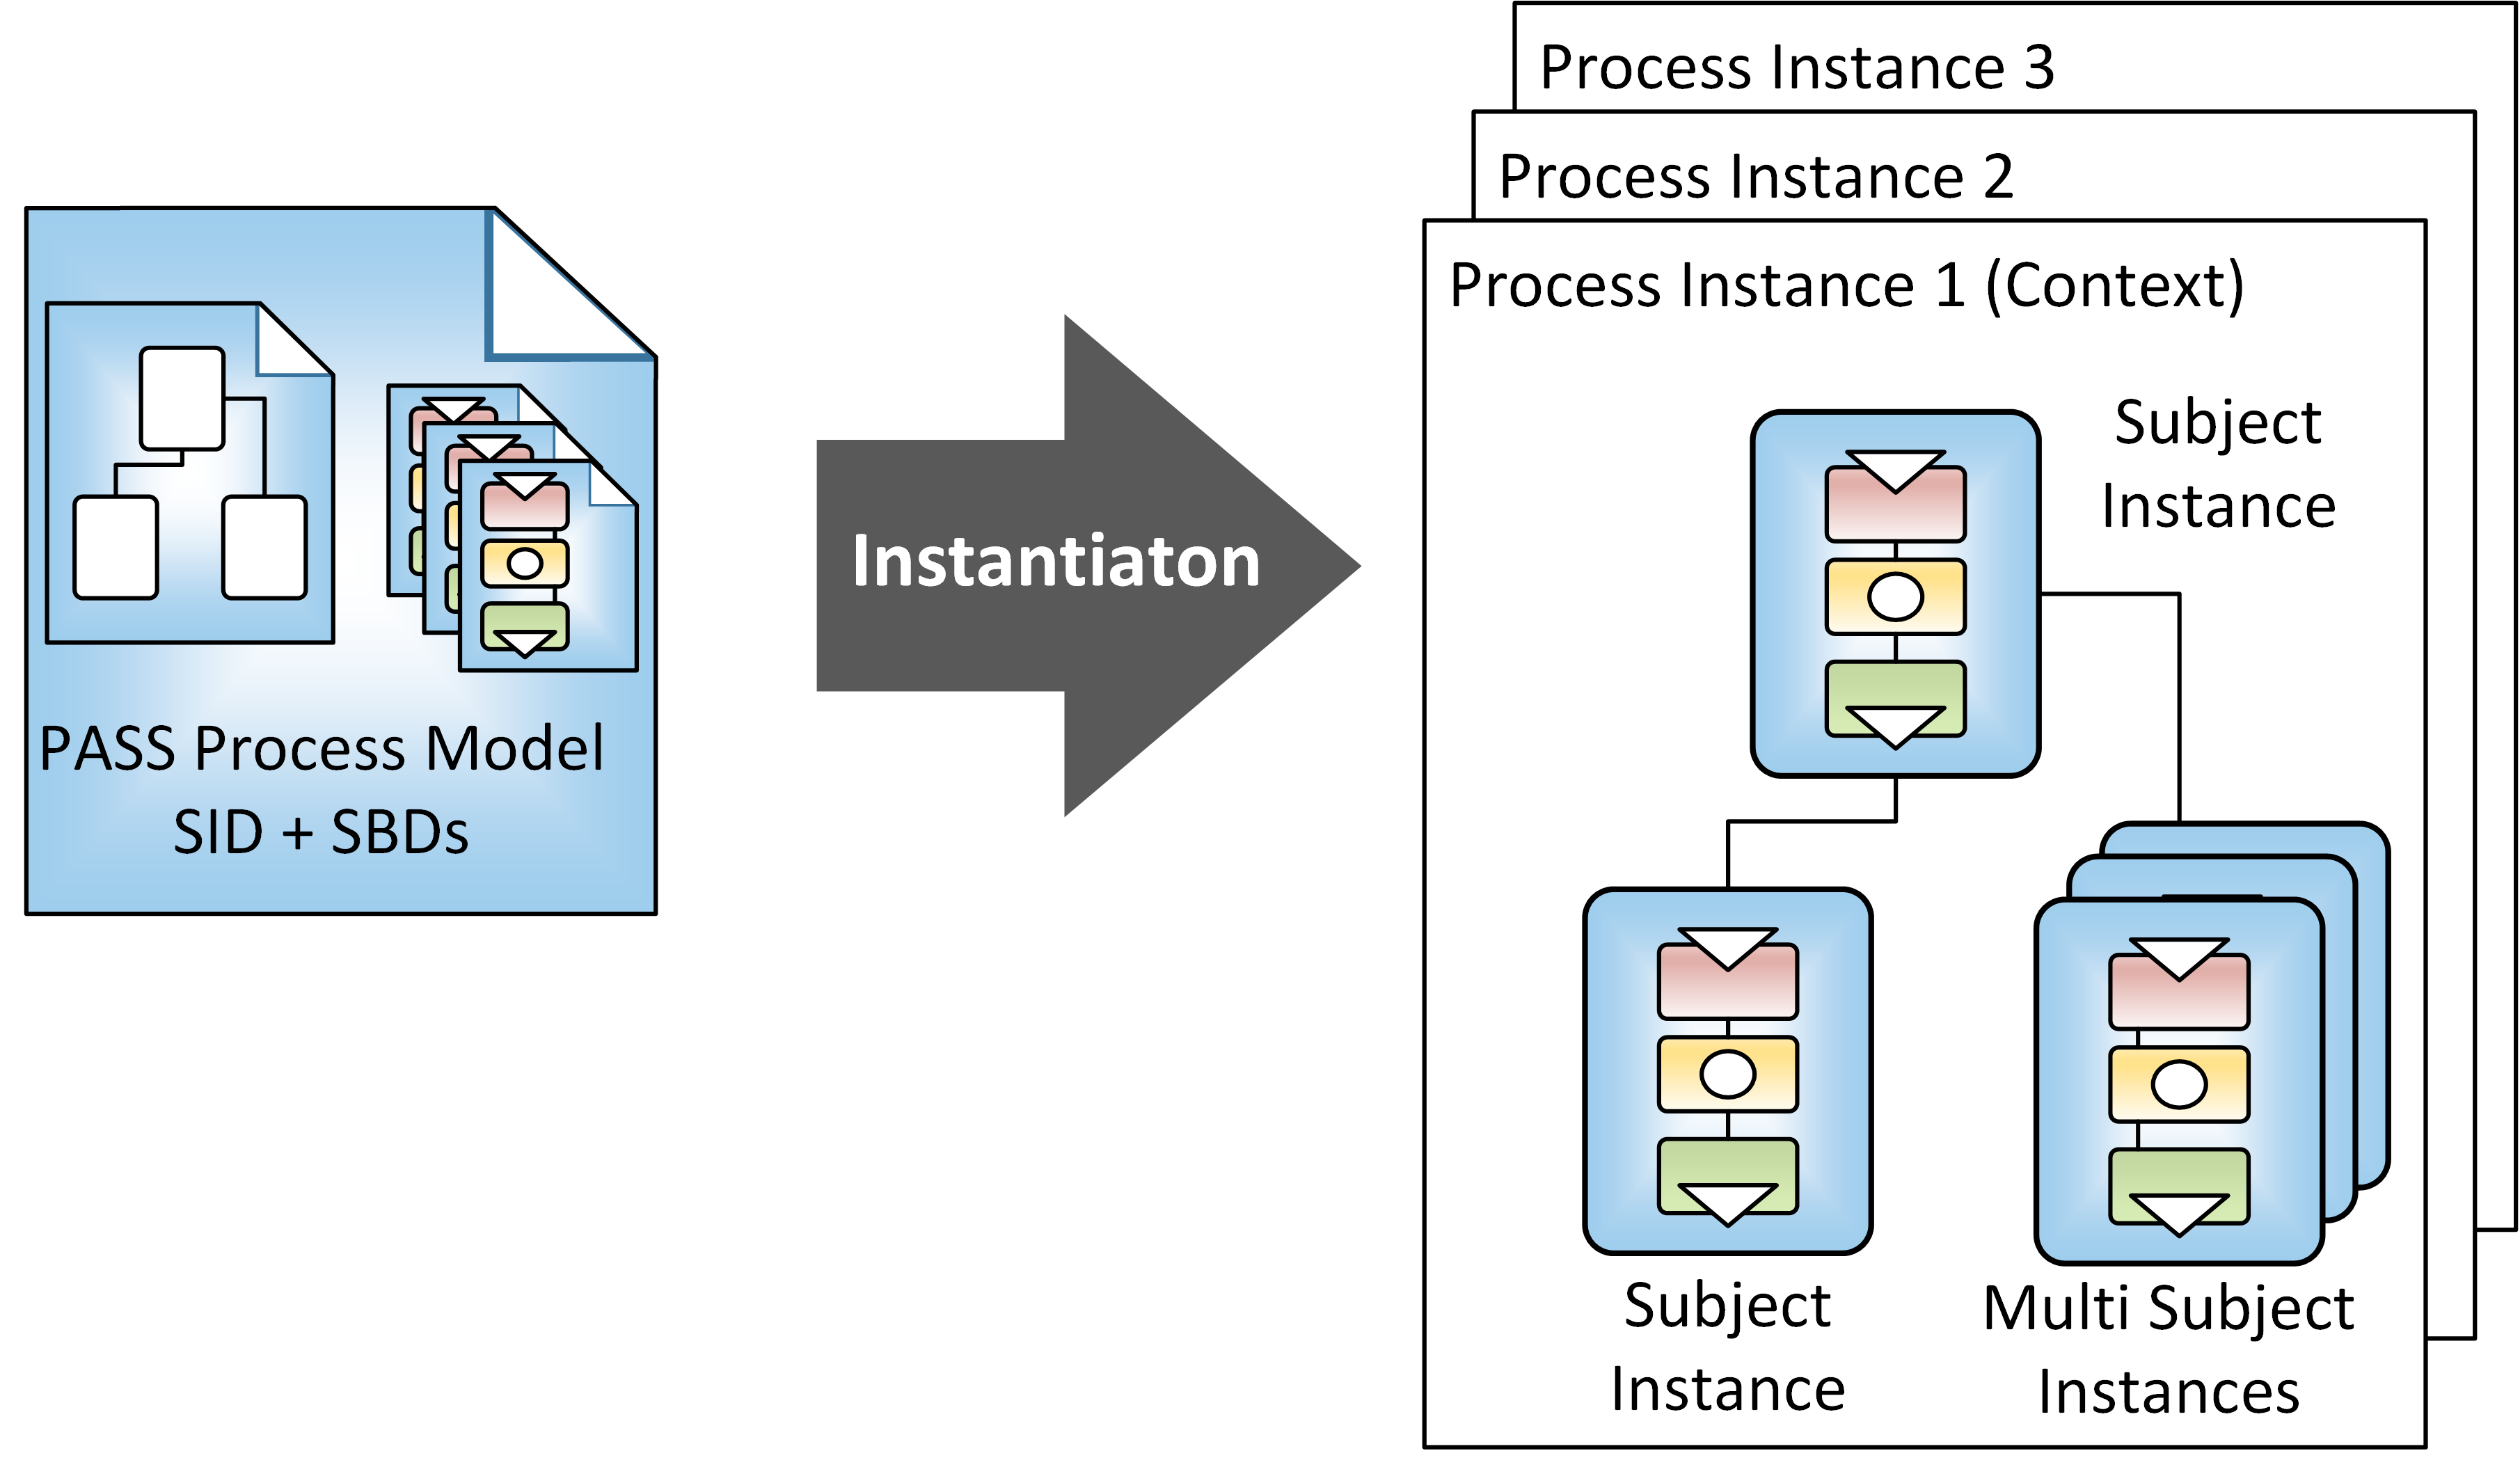
\includegraphics[width=0.9\linewidth]{Figures/PASSExecutionConceptModelAndInstance.png}
	\caption[PASS Process Models in Relation to Process (Model) Instances and Subject Instances]{PASS Process Models in Relation to Process (Model) Instances and Subject Instances}
	\label{fig:processModelInstance}
\end{figure*}

The sub-division between Process Instances and Subject Instances allows the distinction between the termination of the overall process instances or context from the ending of an individual subject instance. As described in the discussion of End States in section \ref{sec:endStates}, in principle, a subject-is allowed to exit an end state again if modeled so. This only make sense if the overall process context has not yet ended and also requires a concept of when this is not possible anymore. In consequence, the meaning of a Subject Instance being \textit{"in an End State"} of its Behavior is different from a Subject Instance being \textit{"terminated"}. The understanding is, that a Subject Instance can only be terminated when all other Subject Instances in the context of the same process instance are also in an End State.


\begin{figure*}[htbp]
	\centering
	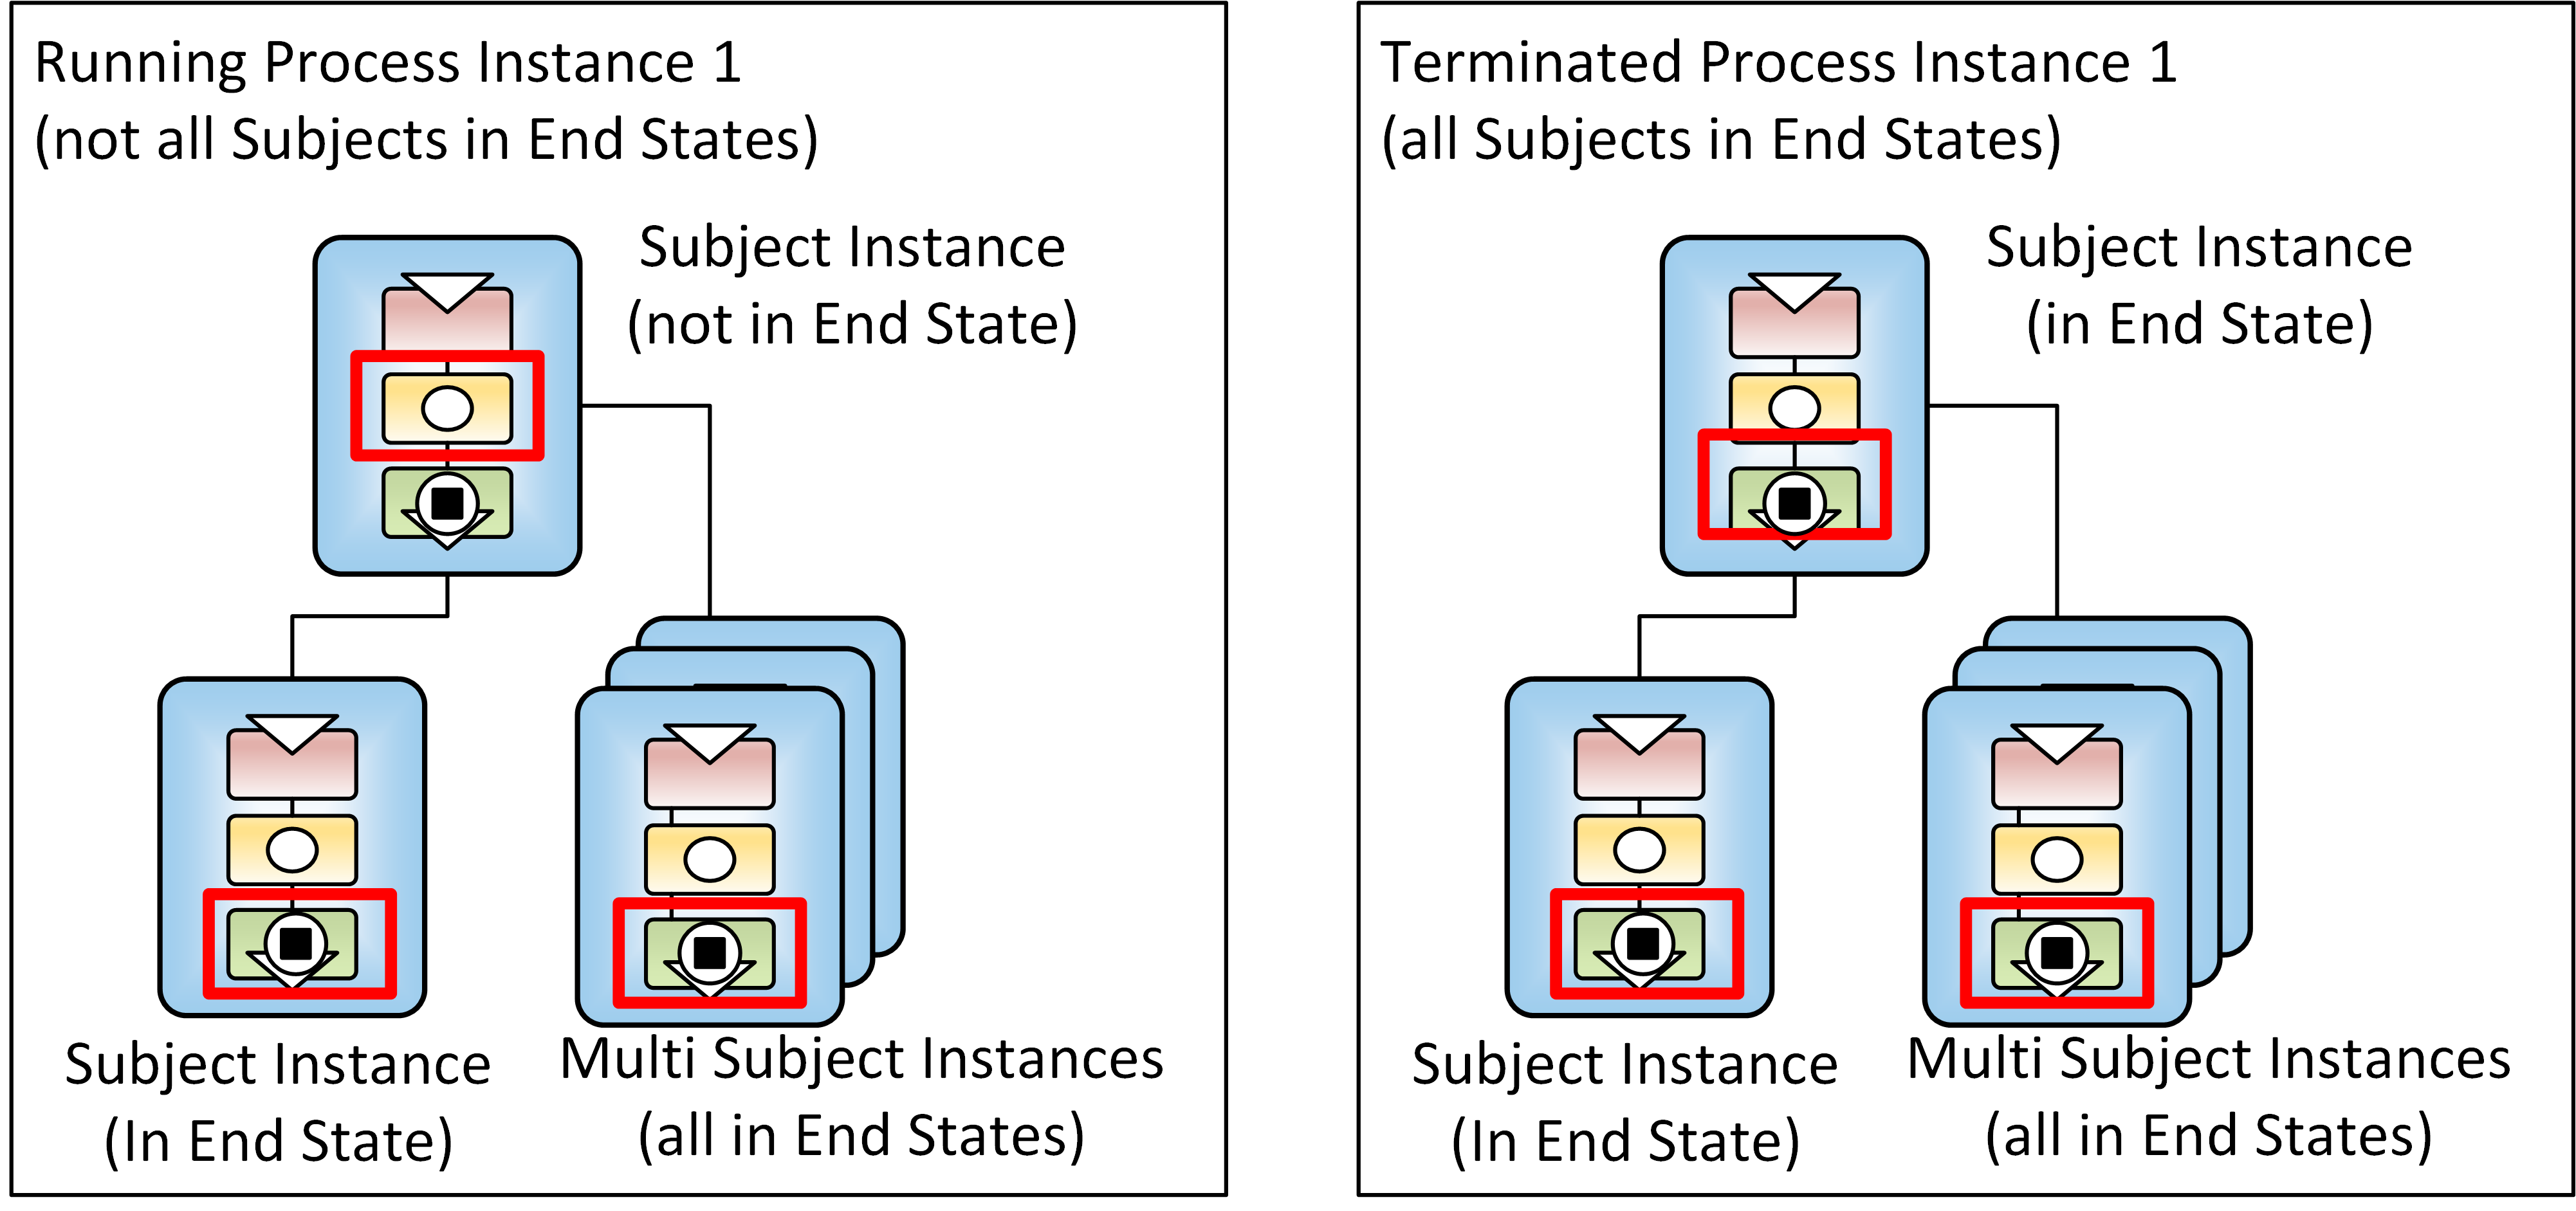
\includegraphics[width=0.9\linewidth]{Figures/PASSExecutionConceptIntanceTermination.png}
	\caption[Conceptual Depiction of running and terminated process/subject intances]{Conceptual Depiction of running and terminated process/subject intances}
	\label{fig:runningAndTerminatedInstances}
\end{figure*}


\subsubsection{Subjects Instances, Subject Carriers, and Inboxes}
\label{sec:subjectCarrier} 

As stated in Section \ref{sec:InputPoolRestrictions} on Input Pool Restrictions, during execution, each Subject Instance is considered to haven Input Pool or Inbox for the Messages. This Inbox is bound to the Subject Instance and not to the person or technical entity that is responsible for executing the instance's behavior.

This entity that \textit{"drives"} the execution of a Subject's Behavior is called the \textbf{Subject Carrier} or Processor. The idea of the subject carrier is a general concept and could imply a real person as well as an automated technical system. Within the bounds of an IT-Workflow system, a human being or other real-world entity would necessarily require an according (graphical user) interface (GUI) to make updates to the execution status that is tracked inside the workflow software.

This differentiation between "Subject Carrier" and "Subject" is important to understand PASS and also the terminology of why the model element is called a "Subject". First and foremost, the idea helps to understand that in the Subjects in a process model describe abstract, process specific roles and not the activities of concrete entity. That real life entity, e.g. the manager in a company, can take control of different Subject Instances in different processes. E.g. he can be responsible for the manager subject in the Business Trip Organisation process for his own staff, while for his own business trips he takes on the role the applicant subject with his own superior.

\begin{figure*}[htbp]
	\centering
	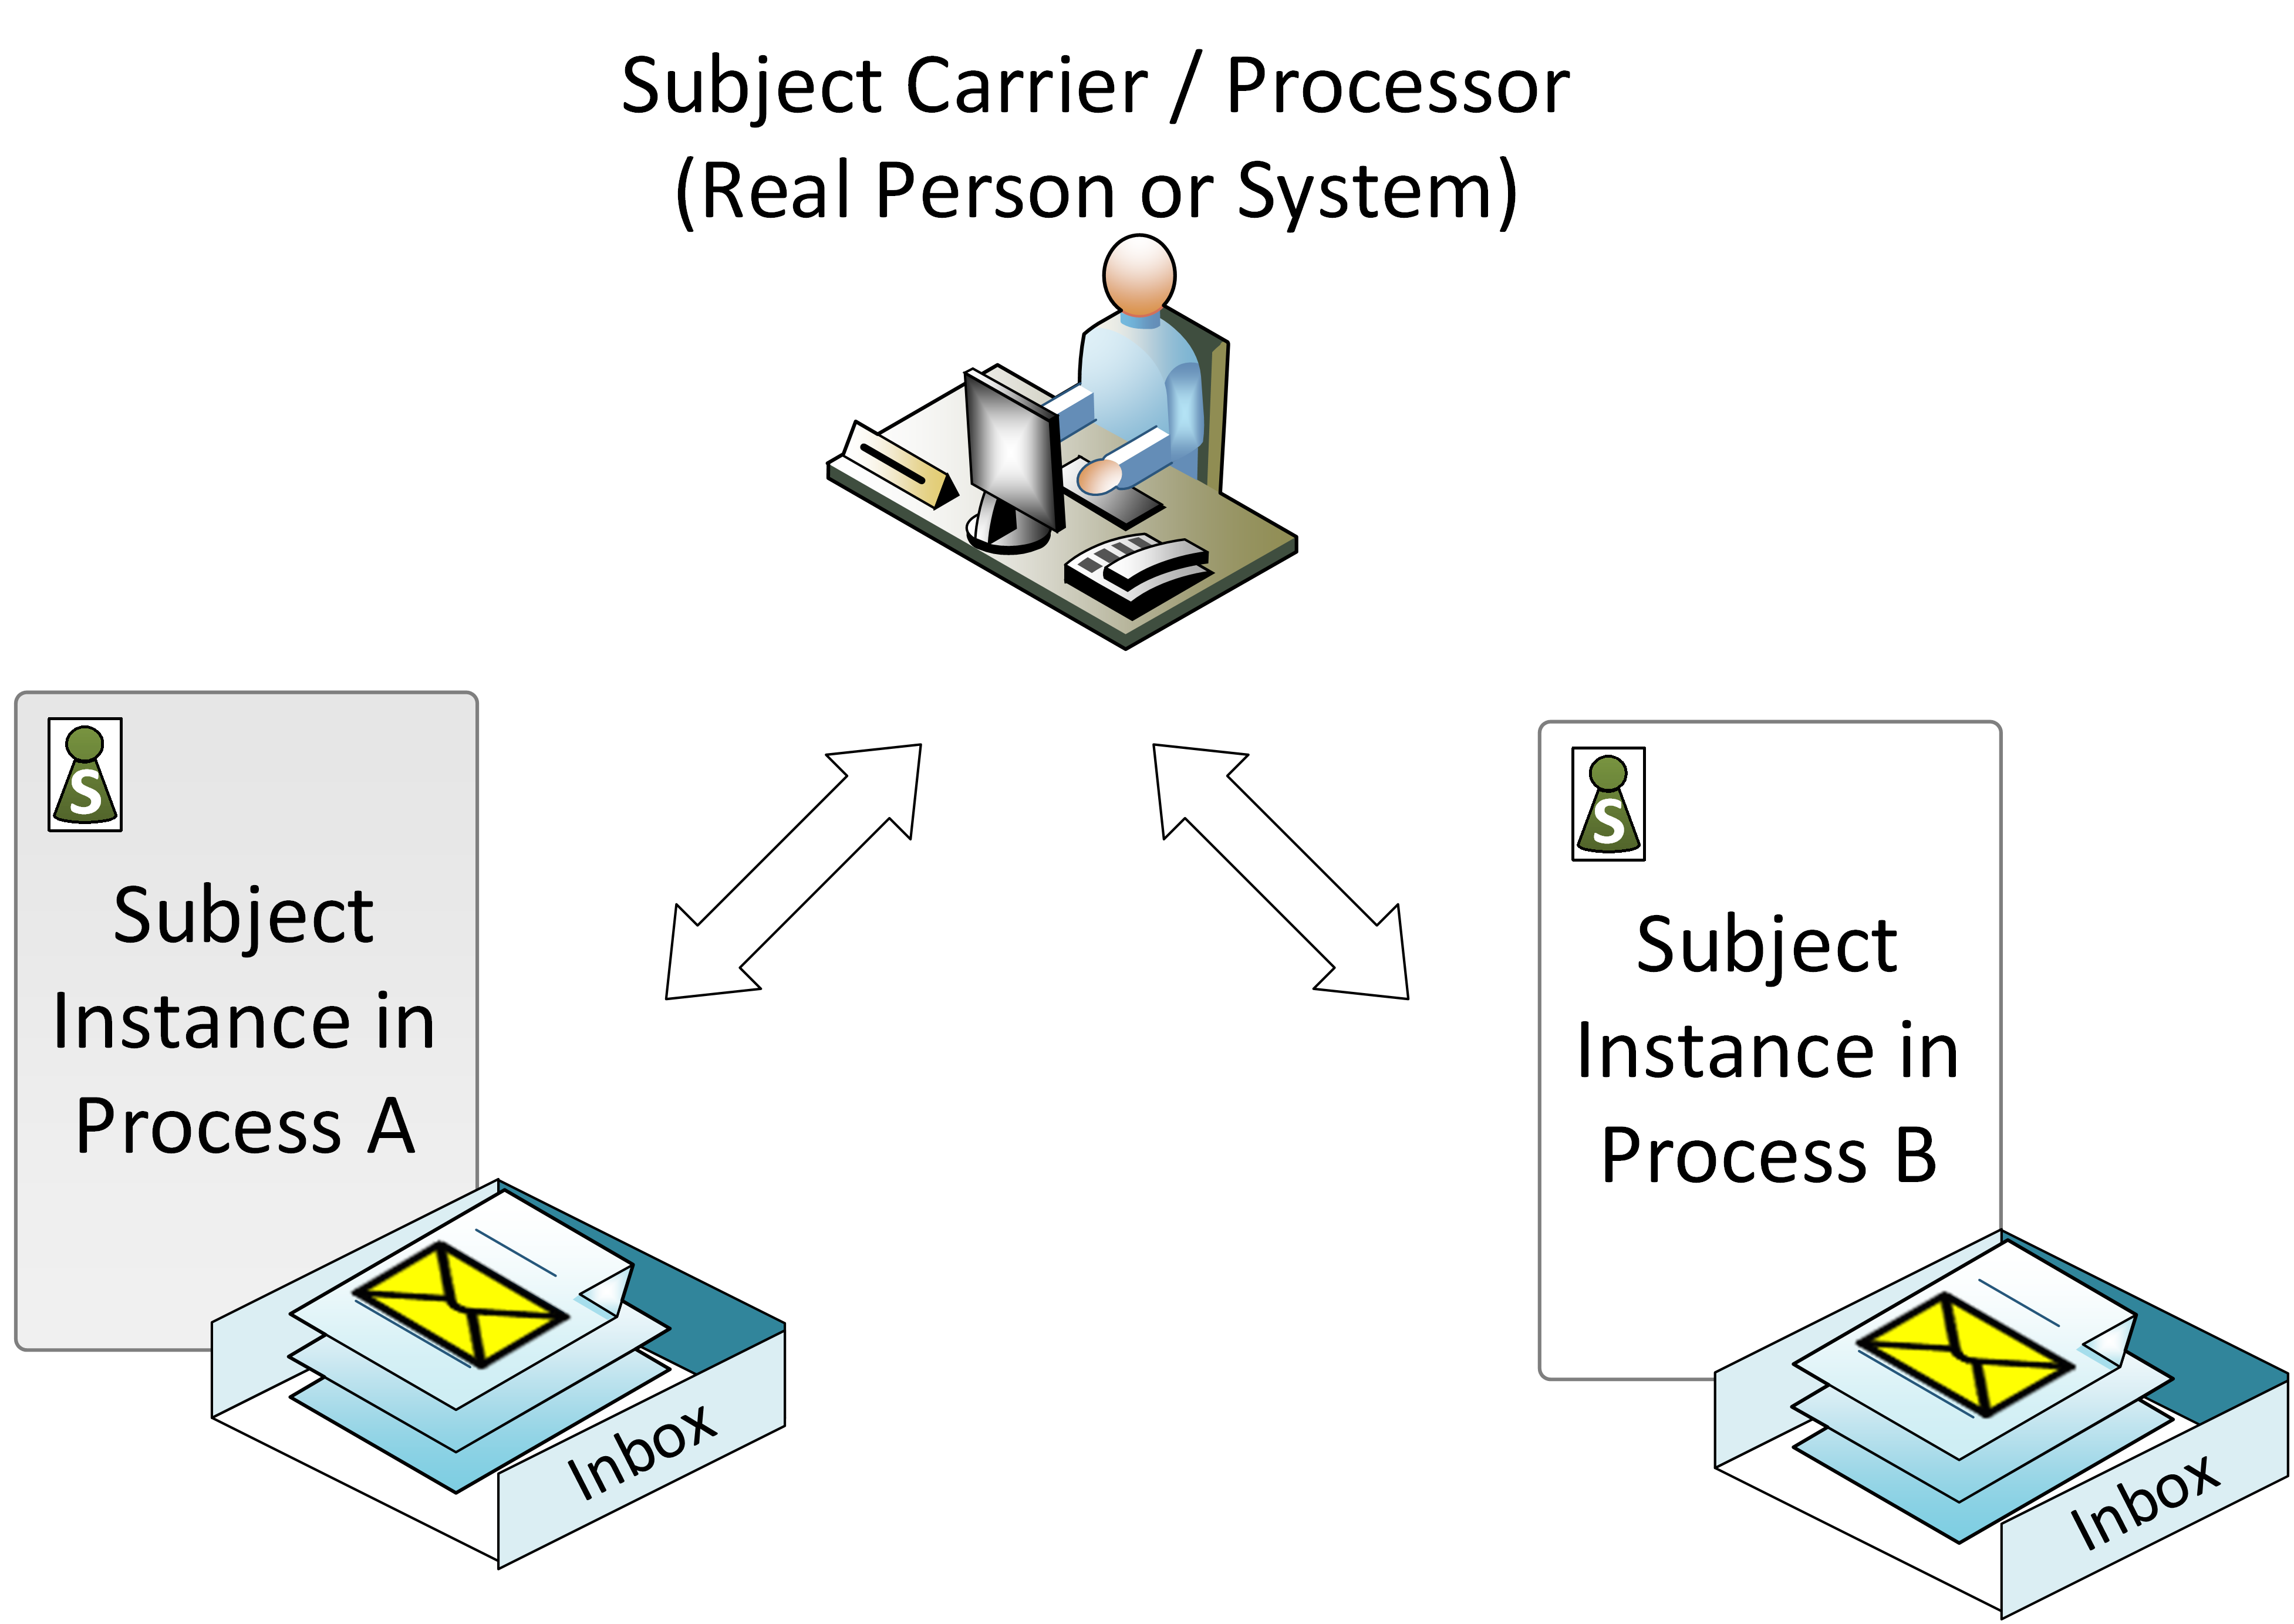
\includegraphics[width=0.6\linewidth]{Figures/SubjectCarrierConcept1.png}
	\caption[Concept of one Subject Carrier(processor) responsible for multiple Subjects in different process, each with its individual inbox (\cite{elstermann:diss})]{Concept of one Subject Carrier(processor) responsible for multiple Subjects in different process, each with its individual inbox(\cite{elstermann:diss})}
	\label{fig:subjectCarrierConcept1}
\end{figure*}

Equally, the subject carrier of a single subject could change during the execution of a behavior. The possibility to switch and the according management is part of the functionality of an execution engine and not per-se of the model itself. Currently the PASS modeling standard has no specific mechanism to limit or encourage subject carrier switching.

\begin{figure*}[htbp]
	\centering
	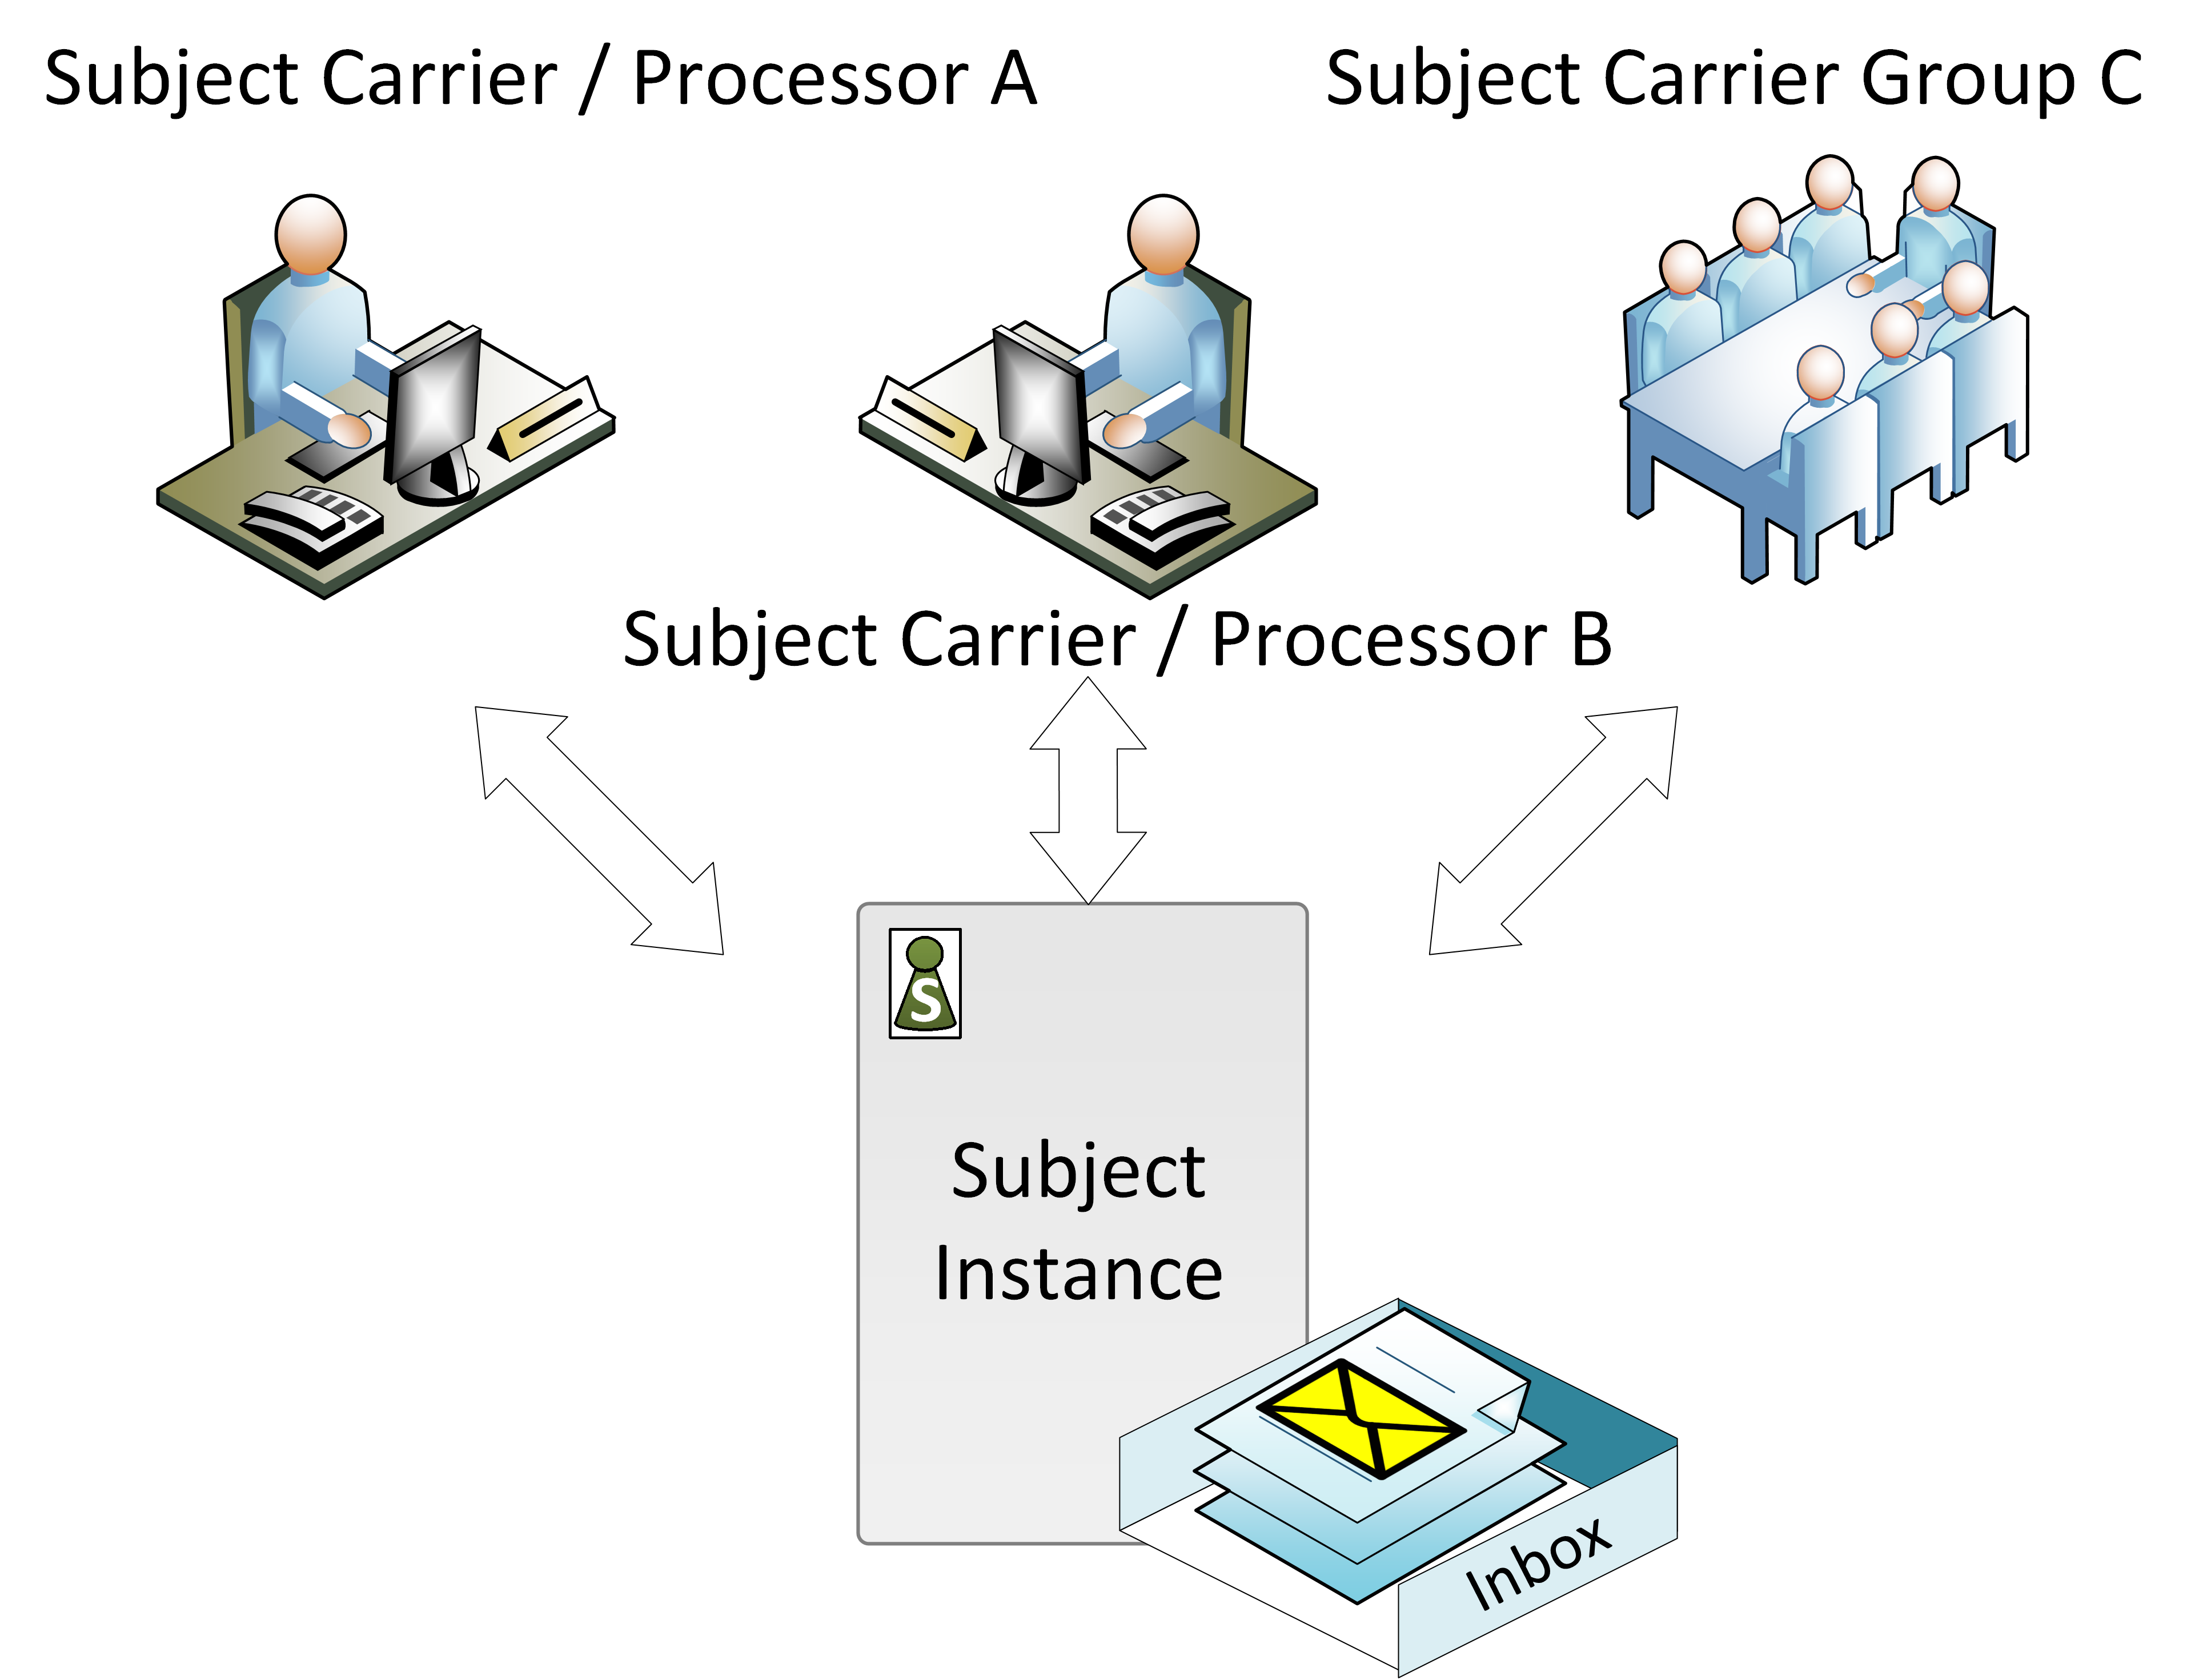
\includegraphics[width=0.6\linewidth]{Figures/SubjectCarrierConcept2.png}
	\caption[Concept of multiple Subject Carriers (processors) that can alternate in the the execution of on subject instance in a process (\cite{elstermann:diss})]{Concept of multiple Subject Carriers (processors) that can alternate in the the execution of on subject instance in a process (\cite{elstermann:diss})}
	\label{fig:subjectCarrierConcept2}
\end{figure*}

\subsubsection{The Subject vs. Subject Carrier vs. Role vs. Actor vs. Agent}

%ME: admittadly this section currently is pretty much rambling....if someone could find a more formal approach for this important discussion it would be great.

The previous section introduced the concept Subject Carrier as something different from a Subject. Further in the wide field of Computer Science, Business Process Modeling, and IT-System theory, the very similar terms of Actor, Agent, or Role are being used in slightly different but at the same time very similar context to the one here that describes the domain of subject-oriented process modeling with PASS. Often, when learning PASS, people familiar with the mentioned terms wonder how things are related, or if subjects could be called or understand as actors or roles. 
A full discussion of this topic would require an in-dept discussion of each term and the, supposedly impossible, attempt to find a generally accepted and fitting description for especially the terms of role, actor, and agent. 

All of them, including the term of Subject and Subject Carrier, have in common that they refer to or describe something that is an active entity in a specific context. To what degree however differs vastly and depends on the persons understanding for each term. 

In the context of PASS, as stated, "Subject" always refers to the element of a process model for whom it is modeled of how it interacts and what behavior it has in a process context. This is very similar to the concept of "role" often used in IT-system management, where for the purpose of giving users certain rights, they often are assigned to certain groups that in turn can take on certain roles. Due to the similarity the concept of role can easily be matched to Subjects in according workflow systems; they may even use the same labels such as 'Manager'. However, the term role has per-se nothing to do with subject-oriented process models and therefor cannot be used synonymously.

The term "actor" can also be used very similar to the term "Subject", and certain modeling SO modeling environments actually prefer it to the term of Subject (Namely the Act'n'Connect modeling tool). It could be argued, that the term actor is more easily understood as an active entity than the term Subject, where subject could also be understood as being a synonym for "topic" instead of referring to the grammatical structure. On the other hand, actor is very generic term and terminology wise makes it hard to differ "actor" as an specific model element from the concept a general active entity e.g. a real-life actor.

An "agent", or "software agent" is an active entity that could also be described as an actor. However, usually a software agent refers to a individual piece of instruction/or code that runs in specific program context. The activities or behavior of software agent is usually described in program code. While a piece of software referred to as an agent could be responsible for executing a Behavior described in a PASS process model, this is only possibility and illustrates how agent and subject are referring to the same concept.

\subsection{Behavior Execution}

As stated before, an SBD consist of States and Transitions used to describe what actions a subject performs in what order. The execution concept is, that a subject always \textbf{"is in exactly on state"}.  To "be in a state" expresses that the subject is continuously performing the activity described for that state. The activity of state should be denoted at least by its label, but can also be detailed out with a Function Specification. One or more outgoing transition arrow denotes the next possible state to be executed as well as the condition (\textbf{Transition Condition}) that must be fulfilled in order to  follow the denoted path.  


%The blocking of subjects when attempting to send can be monitored over time with the so-called timeout. The example in Figure \ref{fig:sendstatetimer} shows with 'Timeout: 24 h' an additional state transition which occurs when within 24 hours one of the two messages cannot be sent. If a value of zero is specified for the timeout, the process immediately follows the timeout path when the alternative message delivery fails.
\subsubsection{Sending Messages}

Before sending a message, the values of the parameters to be transmitted need to be determined. In case the message parameters are simple data types, the required values are taken from local variables or business objects of the sending subject, respectively. In the case of business objects, a current instance of a business object is transferred as a message parameter.

The sending subject attempts to send the message to the target subject and place it in its input pool. Depending on the described configuration and status of the input pool, the message is either immediately stored or the sending subject is blocked until delivery of the message is possible.


%\begin{figure}[htbp]
%	\centering
%	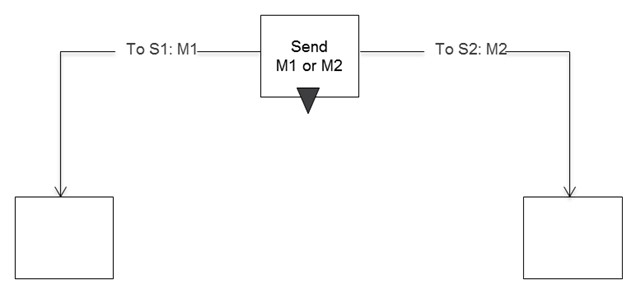
\includegraphics[width=0.7\linewidth]{Figures/Ontology/SubjectBehavior/sendState}
%	\caption[Example of alternative sending]{Example of alternative sending}
%	\label{fig:sendstate}
%\end{figure}

%By specifying priorities, the order of sending can be influenced. For example, it can be determined that the message M1 to S1 has a higher priority than the message M2 to S2. Using this specification, the sending subject starts with sending message M1 to S1 and then tries only in case of failure to send message M2 to S2. In case of message M2 can also not be sent to the subject S2, the attempts to send start from the beginning.

%The blocking of subjects when attempting to send can be monitored over time with the so-called timeout. The example in Figure \ref{fig:sendstatetimer} shows with 'Timeout: 24 h' an additional state transition which occurs when within 24 hours one of the two messages cannot be sent. If a value of zero is specified for the timeout, the process immediately follows the timeout path when the alternative message delivery fails.

%\begin{figure*}[htbp]
%	\centering
%	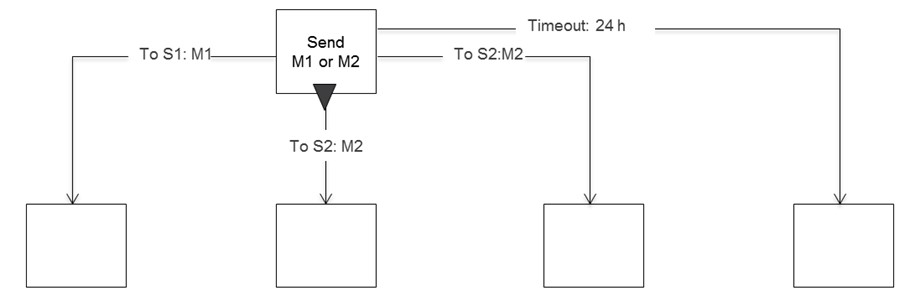
\includegraphics[width=0.7\linewidth]{Figures/Ontology/SubjectBehavior/SendSTateTimer}
%	\caption[Send using time monitoring]{Send using time monitoring}
%	\label{fig:sendstatetimer}
%\end{figure*}

\subsubsection{Receiving Messages}

Analogously to sending, the receiving procedure is divided into two phases, which run inversely to send.

The first step is to verify whether the expected message is ready for being picked up. In the case of synchronous messaging, it is checked whether the sending subject offers the message. In the asynchronous version, it is checked whether the message has already been stored in the input pool. If the expected message is accessible in either form, it is accepted, and in a second step, the corresponding state transition is performed or followed to the next stat. This leads to a takeover of the message parameters of the accepted message to local variables or business objects of the receiving subject. In case the expected message is not ready, the receiving subject is blocked until the message arrives and can be accepted.

In a certain state, a subject can expect alternatively multiple messages. In this case, it is checked whether any of these messages are available and can be accepted. The test sequence is arbitrary unless message priorities are defined. In this case, an available message with the highest priority is accepted. However, all other messages remain available (e.g., in the input pool) and can be accepted in other receive states.

Figure \ref{fig:receivestate} shows a receive state of the subject 'employee' which is waiting for the answer regarding a business trip request. The answer may be an approval or a rejection.

\begin{figure*}[htbp]
	\centering
	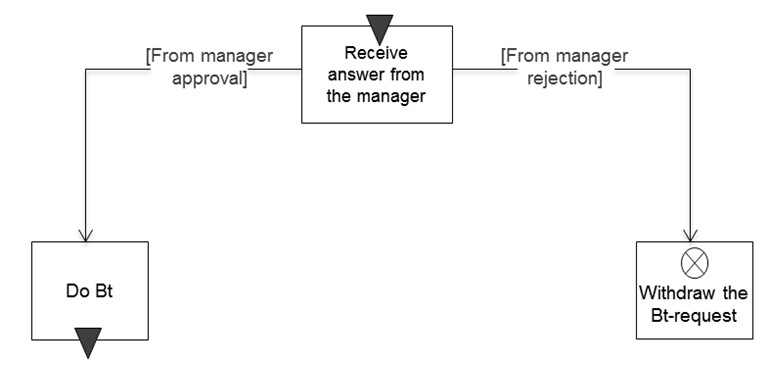
\includegraphics[width=0.7\linewidth]{Figures/Ontology/SubjectBehavior/ReceiveState}
	\caption[Example of alternative receiving]{Example of alternative receiving}
	\label{fig:receivestate}
\end{figure*}

Just as with sending messages, also receiving messages can be monitored over time. If none of the expected messages are available and the receiving subject is therefore blocked, a time limit can be specified for blocking. After the specified time has elapsed, the subject will execute the transition as it is defined for the timeout period. The duration of the time limit may also be dynamic, in the sense that at the end of a process instance the process stakeholders assigned to the subject decide that the appropriate transition should be performed. We then speak of a manual timeout.



\subsubsection{Choice Segment Execution}
\label{sec:choiceSegmentExecution}

In principle a subject can be only in one state at once. The Choice segment may seem as somewhat of a contradiction to that statement, however, it is not. 

There are two possibility interpretations for the execution of this element, a simple and more complex one. 

As an example take a simple Choice segment with three paths, A, B, and C, with A being Mandatory to start and end, B being mandatory to start, and C being optional to start but mandatory to end, as is shown in Figure \ref{fig:choiceSegmentExecution}. 

\begin{figure*}[htbp]
	\centering
	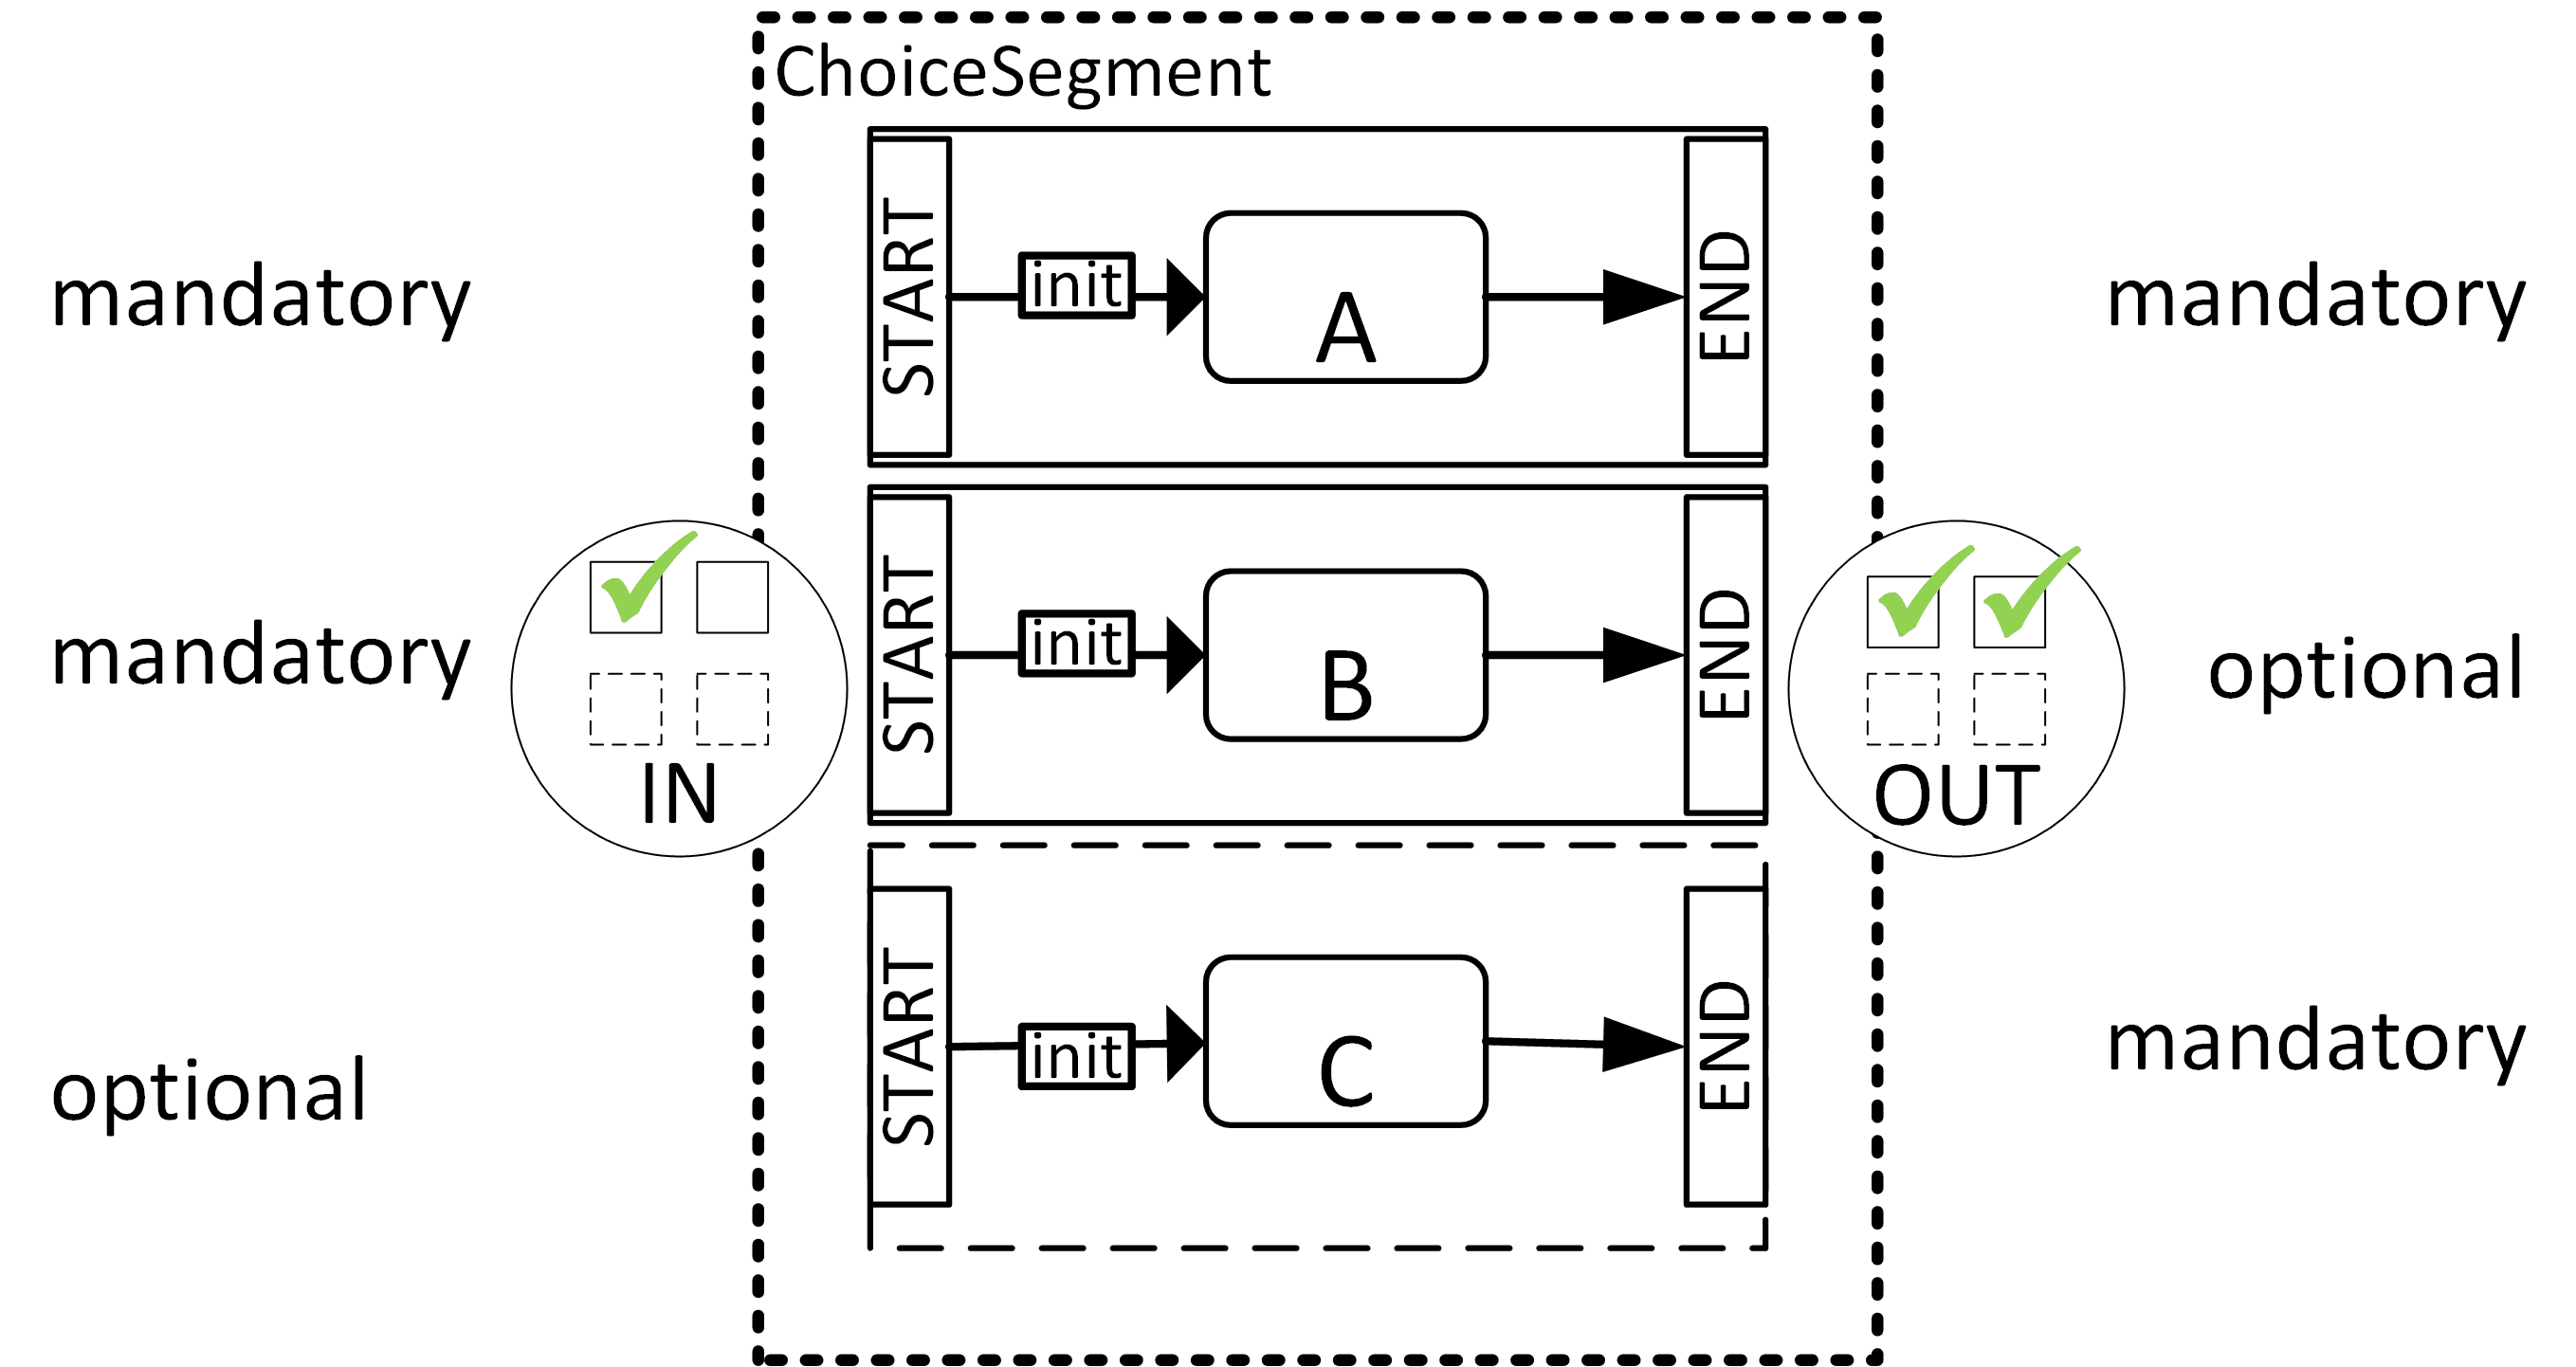
\includegraphics[width=0.7\linewidth]{Figures/Ontology/SubjectBehavior/ChoiceSegment.png}
	\caption[Exemplary Choice Segment with three paths, with different sets of mandatory/optional settings]{Exemplary Choice Segment with three paths, with different sets of mandatory/optional setting}
	\label{fig:choiceSegmentExecution}
\end{figure*}

The simple interpretation is to simply interpret the Choice Segment simply as a short cut or a compact variant to modeling a multitude of possible paths as is shown in figure \ref{fig:choiceSegmentExecutionInterpretation}. Path C can always be circumvented, but once started must be completed. While B cannot be circumvented but can always be  "skipped" out once started. A can't be neither. This interpretation works very well especially for one-state paths. If a path contains more states, or even branching, which is technically allowed, this interpretation becomes somewhat restricting, as any path must first be finished individually after starting, before starting the next path segment. 

\begin{figure*}[htbp]
	\centering
	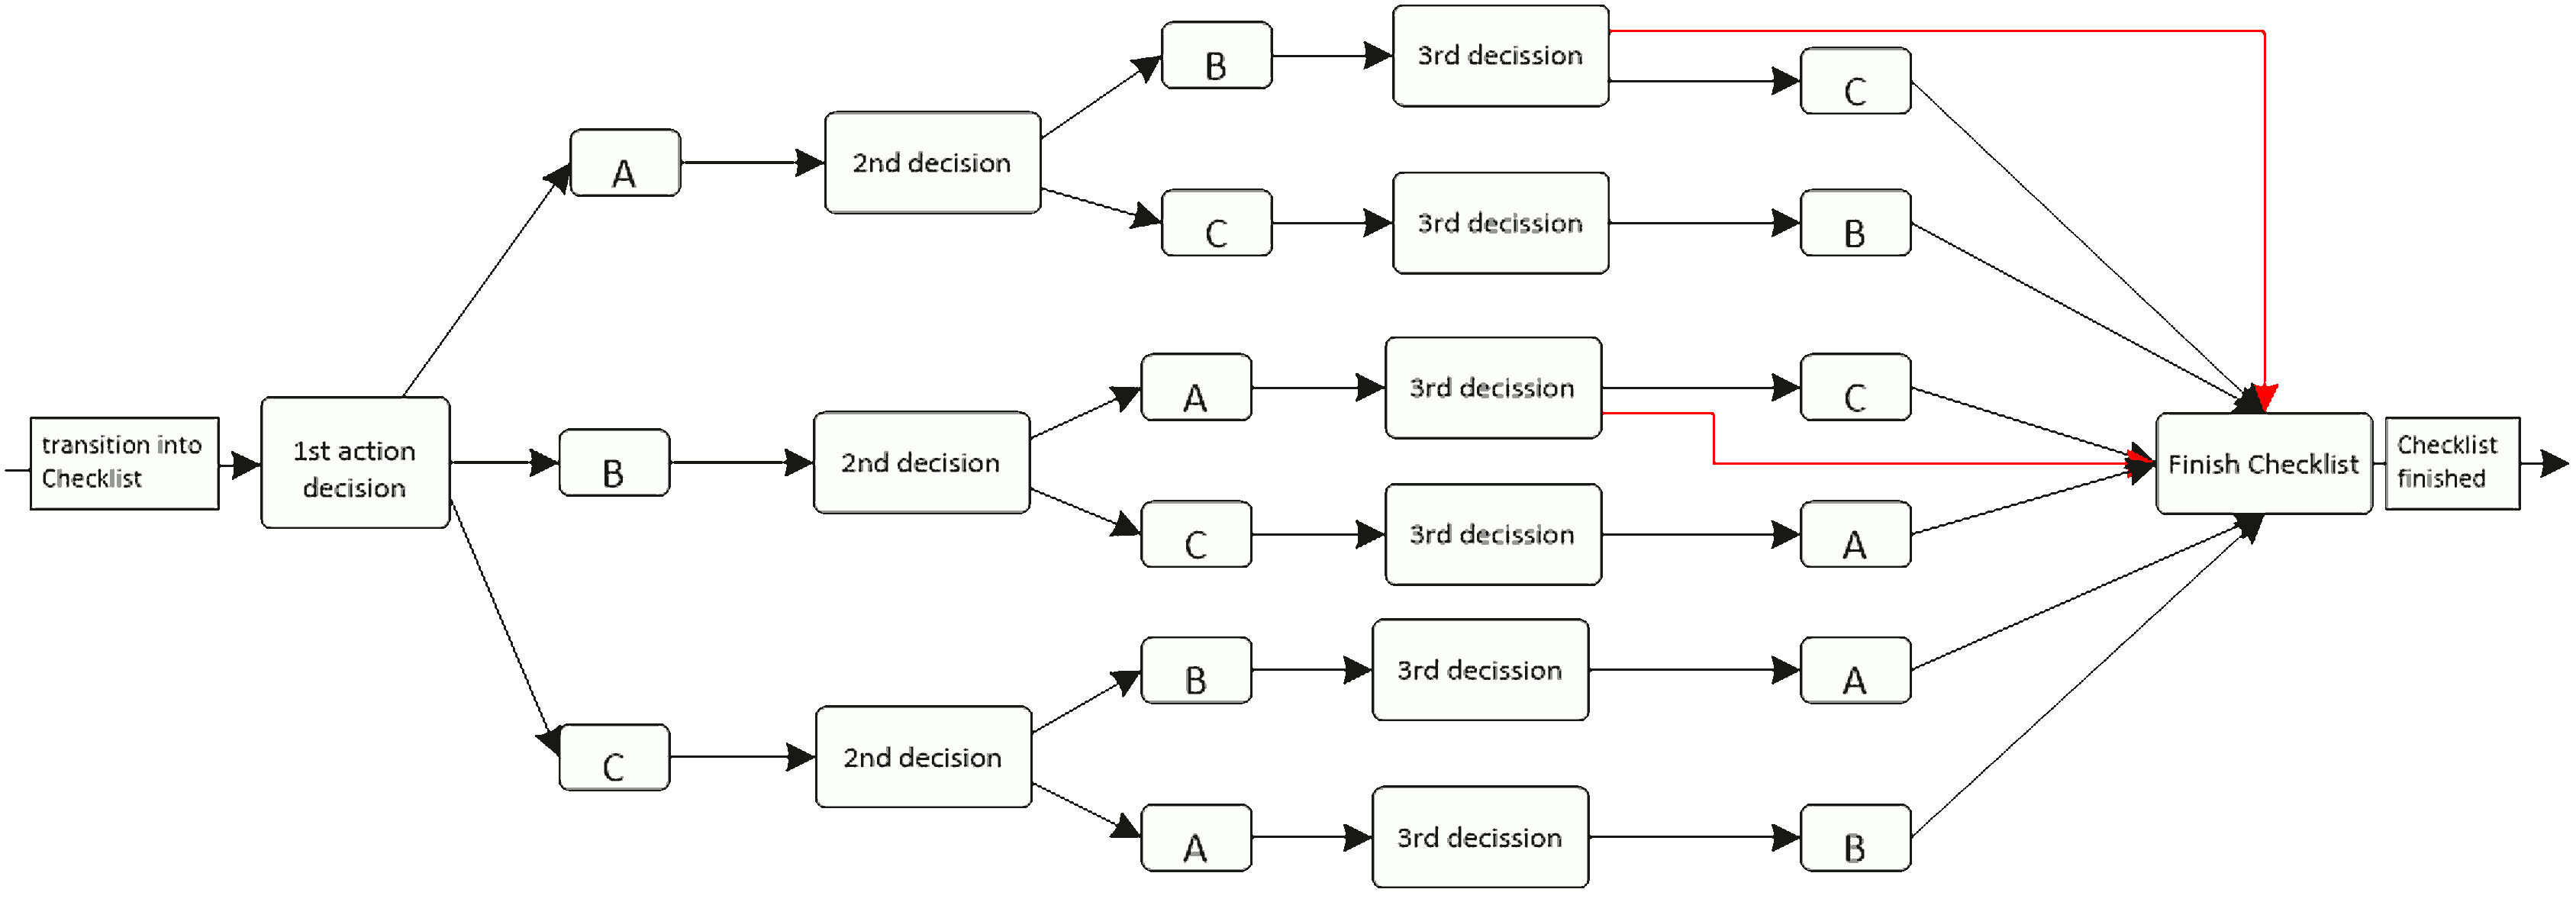
\includegraphics[width=0.9\linewidth]{Figures/Ontology/SubjectBehavior/ChoiceSegmentInterpretation.png}
	\caption[Simple Execution Interpretation of a Choice Segment shown in Figure \ref{fig:choiceSegmentExecution}]{Simple Execution Interpretation of a Choice Segment shown in Figure \ref{fig:choiceSegmentExecution}}
	\label{fig:choiceSegmentExecutionInterpretation}
\end{figure*}

The more complex interpretation of the execution of the Choice Segment does allow switching between the execution of the active state in each separated path upon the arbitrary choice of the subject carrier. However, for that to work, a possible execution engine, in theory, must be able to trace the current state in each path separately and possibly even allow to interrupt the execution of one state temporarily. That would be necessary in order to continue the execution upon the external subject carrier making the choice to switch back to the execution of that path. 


\subsubsection{Default Functions}


\PASSDefaultIndividual{DefaultFunctionDo1\_EnvironmentChoice}
\PASSDefaultIndividual{DefaultFunctionDo2\_AutomaticEvaluation}
\PASSDefaultIndividual{DefaultFunctionReceive1\_EnvironmentChoice}
\PASSDefaultIndividual{DefaultFunctionReceive2\_AutoReceiveEarliest}
\PASSDefaultIndividual{DefaultFunctionSend}


\subsection{Substitutions for Specialized PASS Transition Execution}

In the PASS standard, there are several specialized Transitions. For their execution, they could be interpreted or substituted in the following ways with the standard elements. 

Note that all of these are possible technical substitutions that should allow a standard interpreter to handle these transitions. However, an actual workflow execution engine can implement these elements also in other ways.

\subsubsection{User Cancel Transitions},

To interpret and correctly execute, \PASSModelElement{UserCancelTransition}s, the existence of User or Subject Carrier in an execution software must be assumed. Equally, a technical solution to communicated with this user must be assumed. Consequently, each User-Cancel transition could be substitute as is shown in Figure \ref{fig:usercancelSubstitution}. An additional interface subject needs to be added that connects to an implementation that in turn allows interaction with the user beyond the process flow. 


\begin{figure*}[hp]
	\centering
	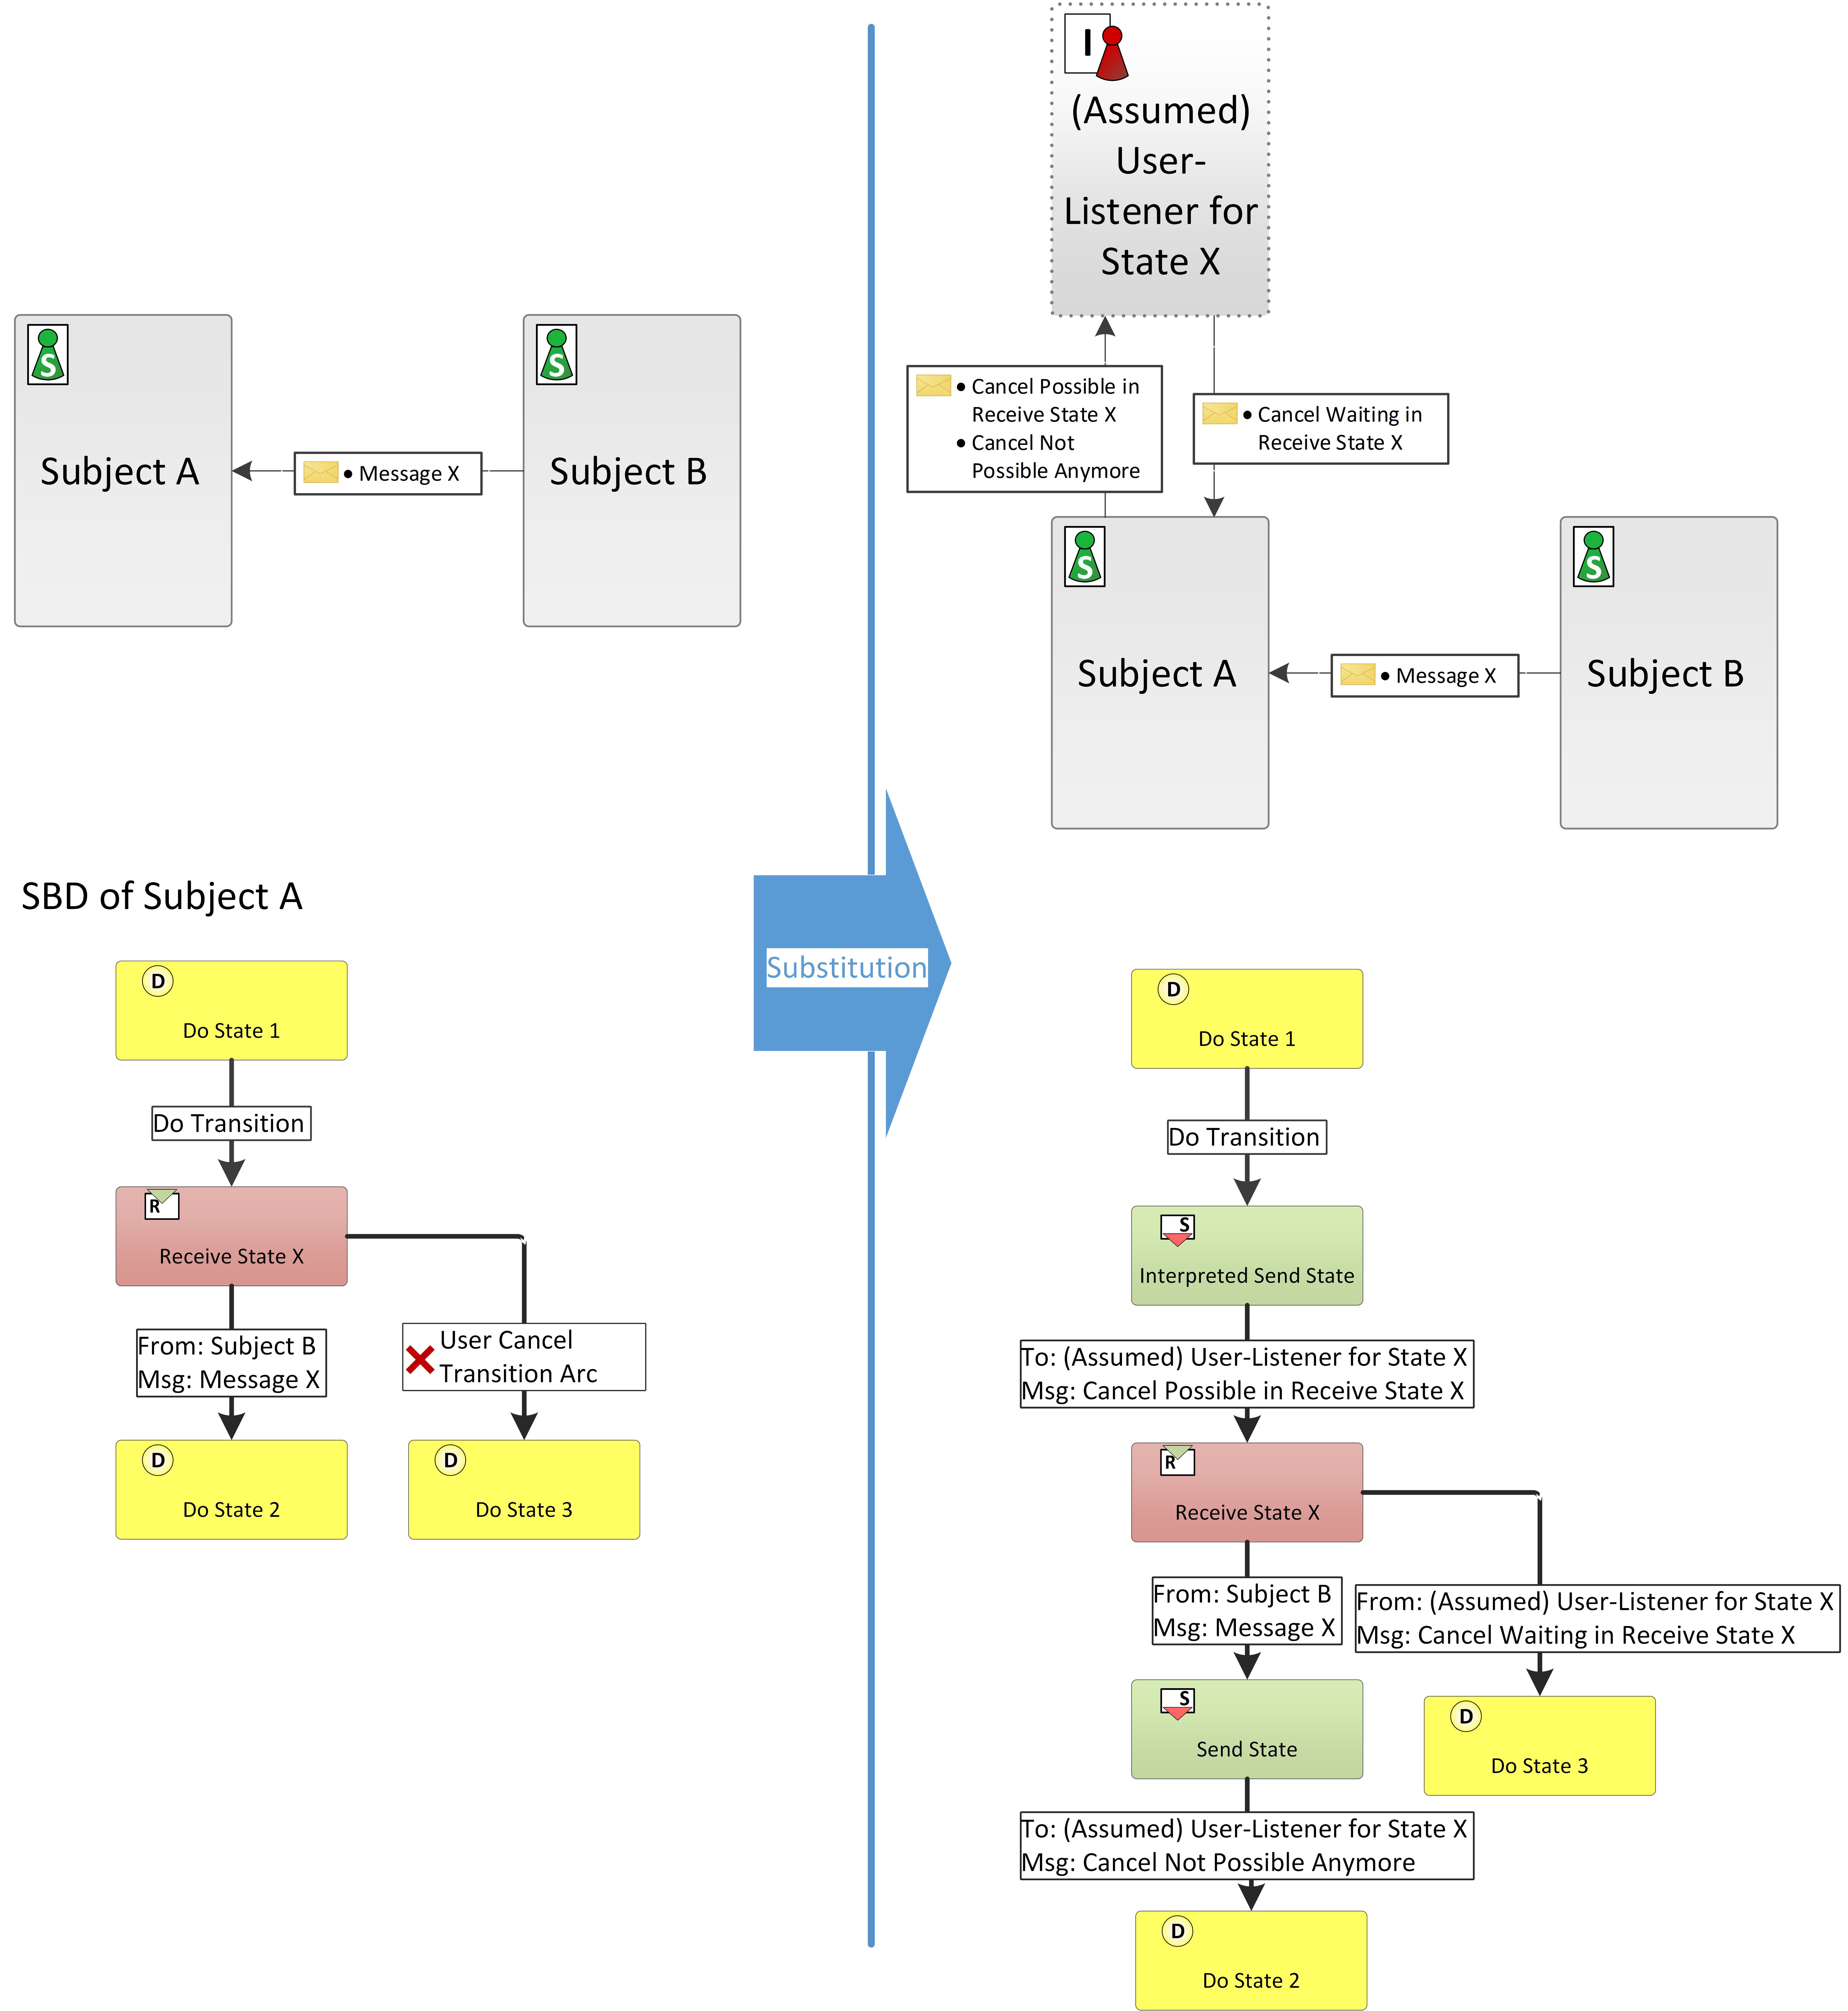
\includegraphics[width=1.0\linewidth]{Figures/Ontology/UserCancelInterpretationSIDSBD.png}
	\caption[Possible Substitution of a \PASSModelElement{UserCancelTransition} for execution]{Possible Substitution of a \PASSModelElement{UserCancelTransition} for execution}
	\label{fig:usercancelSubstitution}
\end{figure*}

Note that this substitution is for User Cancel Transitions originating from Receive States. User Cancel transitions originating from Do States can simply bee seen as relatively specialized Do Transition that allows a user to arbitrarily set the execution of s State Function to be \textit{done}. User Cancels for Send States would need to be substituted similar to a Sending Failed Transition but with the User interacting directly with the Send Controller and deeming a Send activity to be failed.  

\subsubsection{Sending Failed Transitions}
\label{sec:sendingFailedTransitionsExecution}

To interpret \PASSModelElement{Sending Failed Transition}s it is necessary to assume the existence of a technical entity that controls a subject's send activities during execution; the \textit{Send Controller}. After have been given the command to forward a message to a specific subject instance, the send controller does inform a Subject's Behavior Interpreter about a the possible success or failure (after a timeout) and the subject reacts accordingly as depicted in Figure \ref{fig:sendingfailedSubstituion}.


\begin{figure*}[hp]
	\centering
	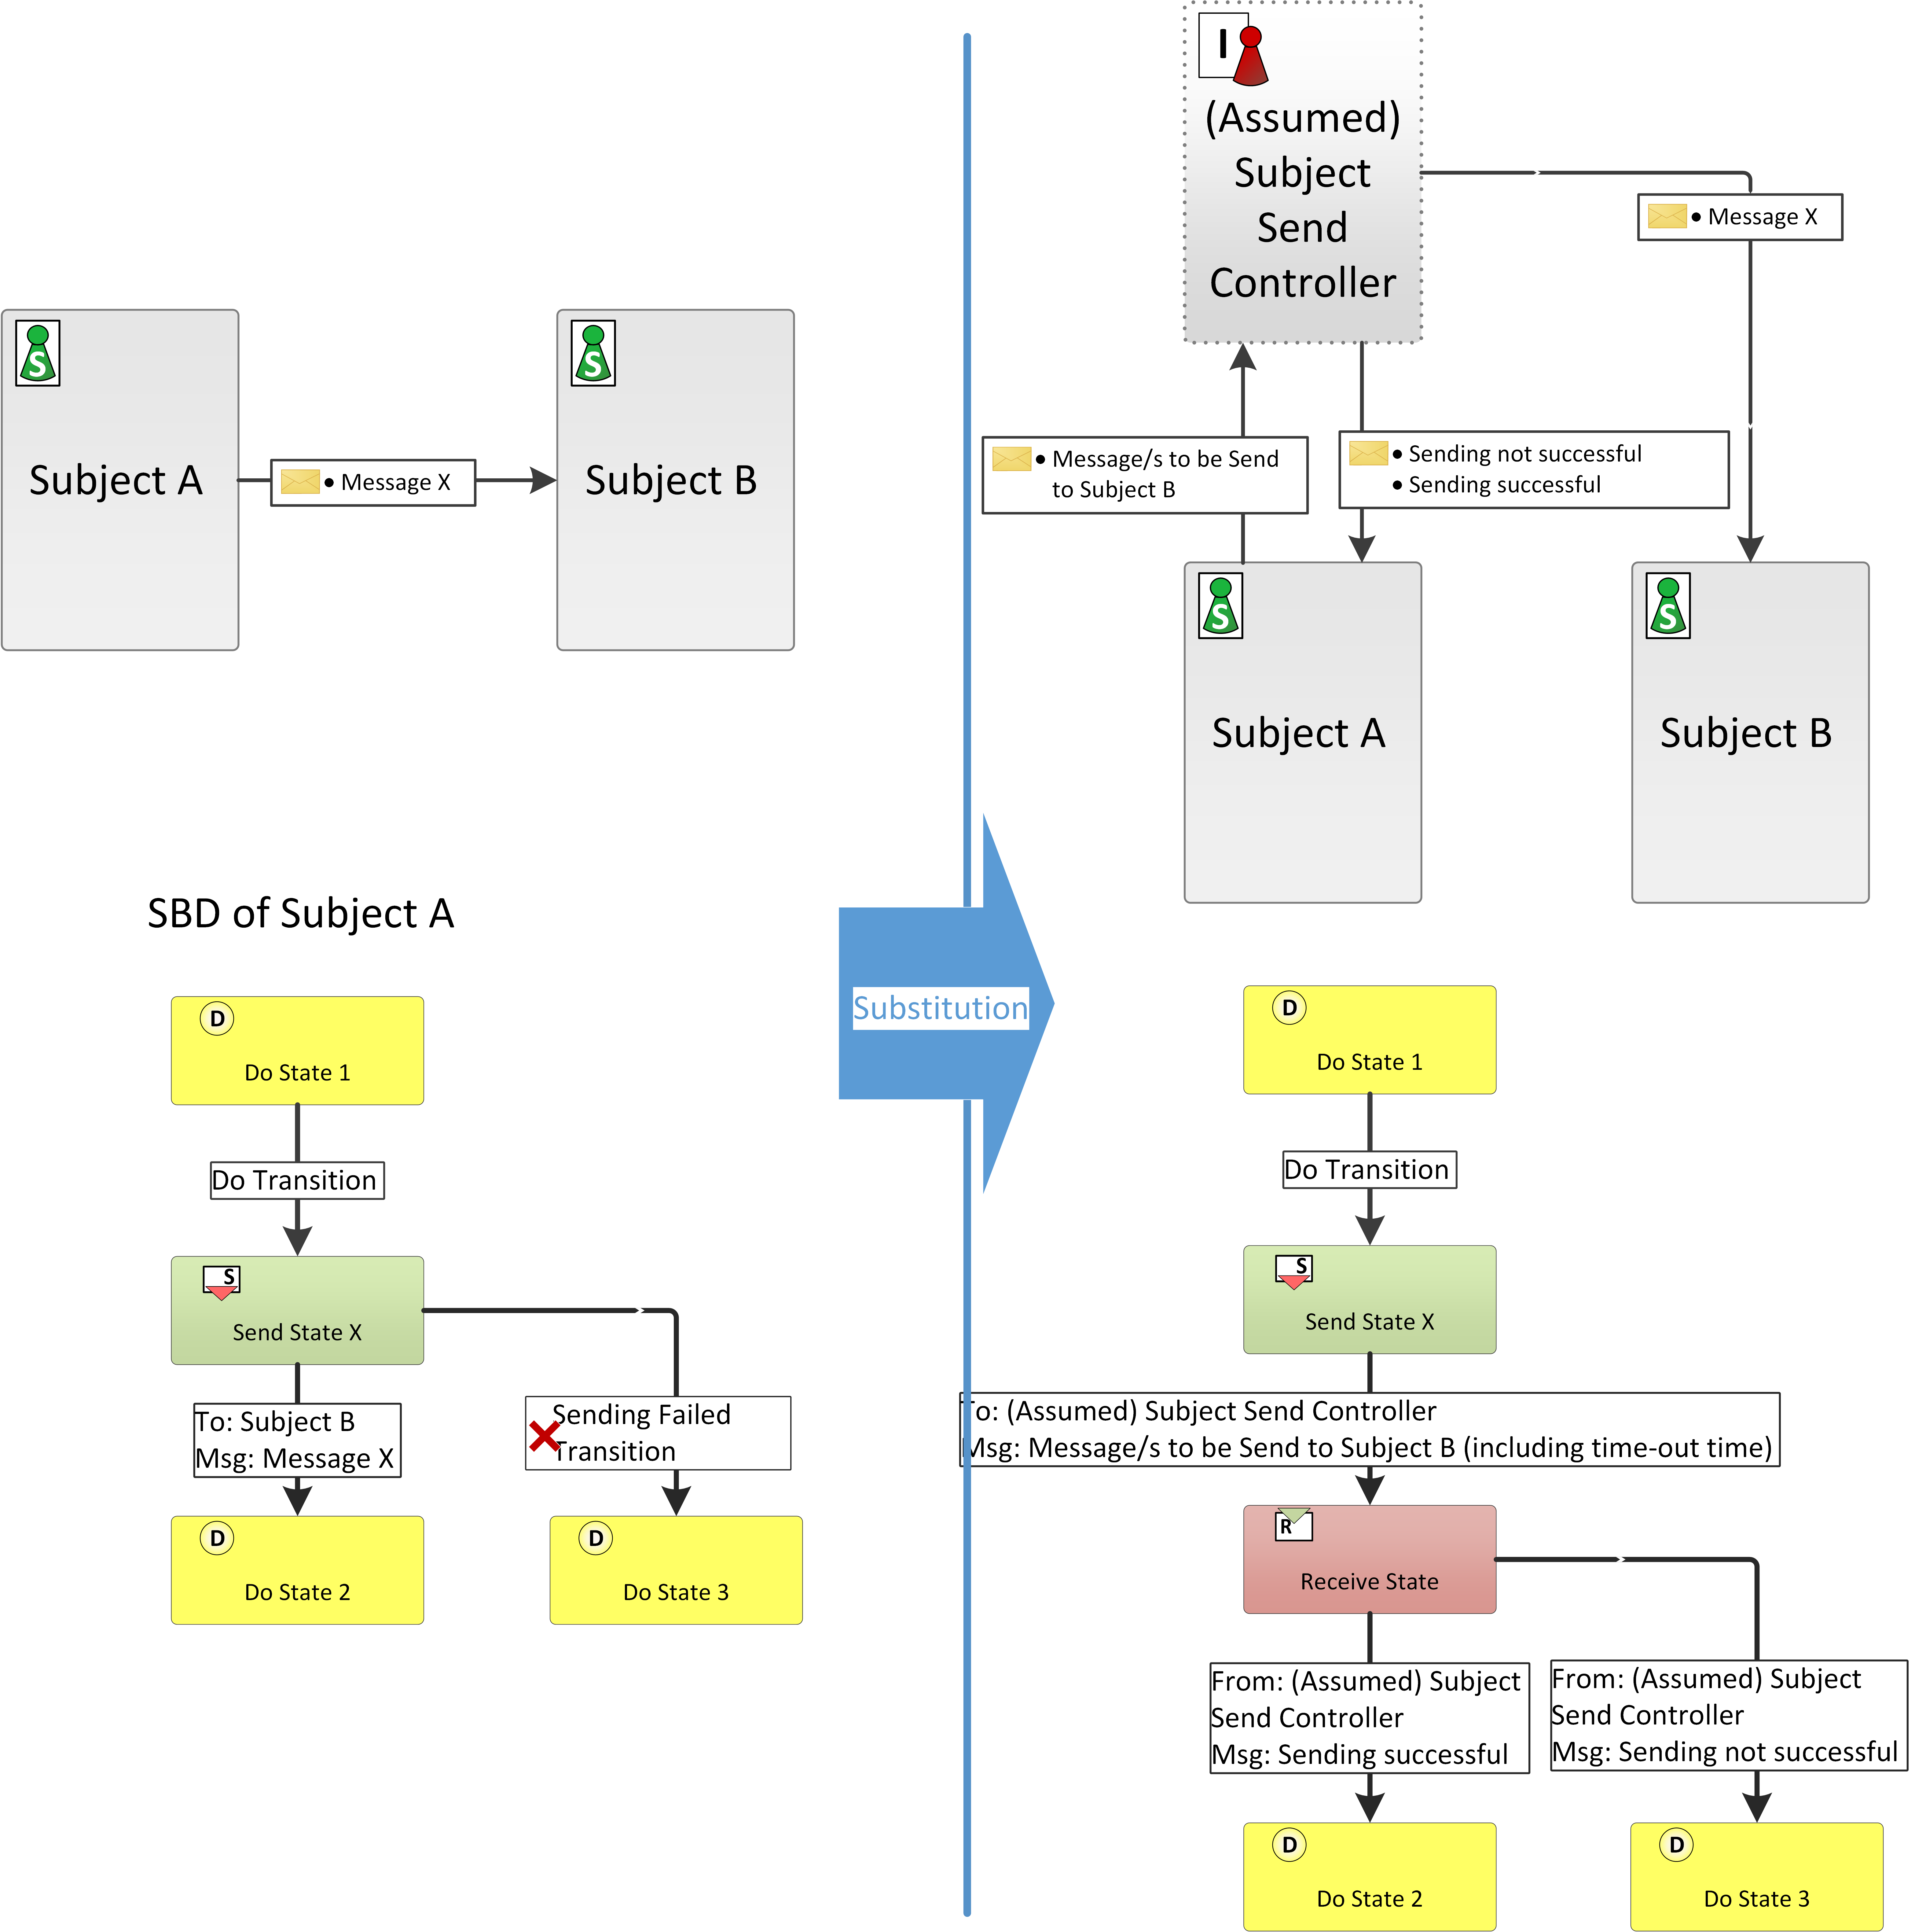
\includegraphics[width=1.0\linewidth]{Figures/Ontology/SendingFailedInterpretationSIDSBD.png}
	\caption[Possible Substitution of a \PASSModelElement{SendingFailedTransition} for execution]{Possible Substitution of a \PASSModelElement{SendingFailedTransition} for execution}
	\label{fig:sendingfailedSubstituion}
\end{figure*}

\subsubsection{Timer Transitions}

There are the two general types of time based transitions:

Substitution  \PASSModelElement{Timer Transition}s and \PASSModelElement{Reminder Transition}. Both work a little different from each other and also different when originating from each of the different state types.

If the execution envoironment is able to handle it, \PASSModelElement{Timer Transition}, also known as \textit{Time-Outs}, can be executed by adding an accordingt time-out funcionallity to a State's internal function.

Otherwise, certain substitutions could be done in order to realizer the execution of Time Transitions. All of them have in common that they require the assumed existence of a timer or calendar subjects that theoretical handles all time calculations and sends an according trigger message when the time has come.

\emph{Timer from Receiver States}

The substitution done for Timer Transitions originating from Receive States. Here, before entering a state with an outgoing timer transition, the according time-out time from that transition needs to be set/send to the timer and the timer transition itself can be substituted simply by another receive transition from that state. If the state can be visited multiple times, the timer will also need to be deactivated. Otherwise, the according time-out message might still be sent and in the subject's inbox when reentering the state.

\begin{figure*}[hp]
	\centering
	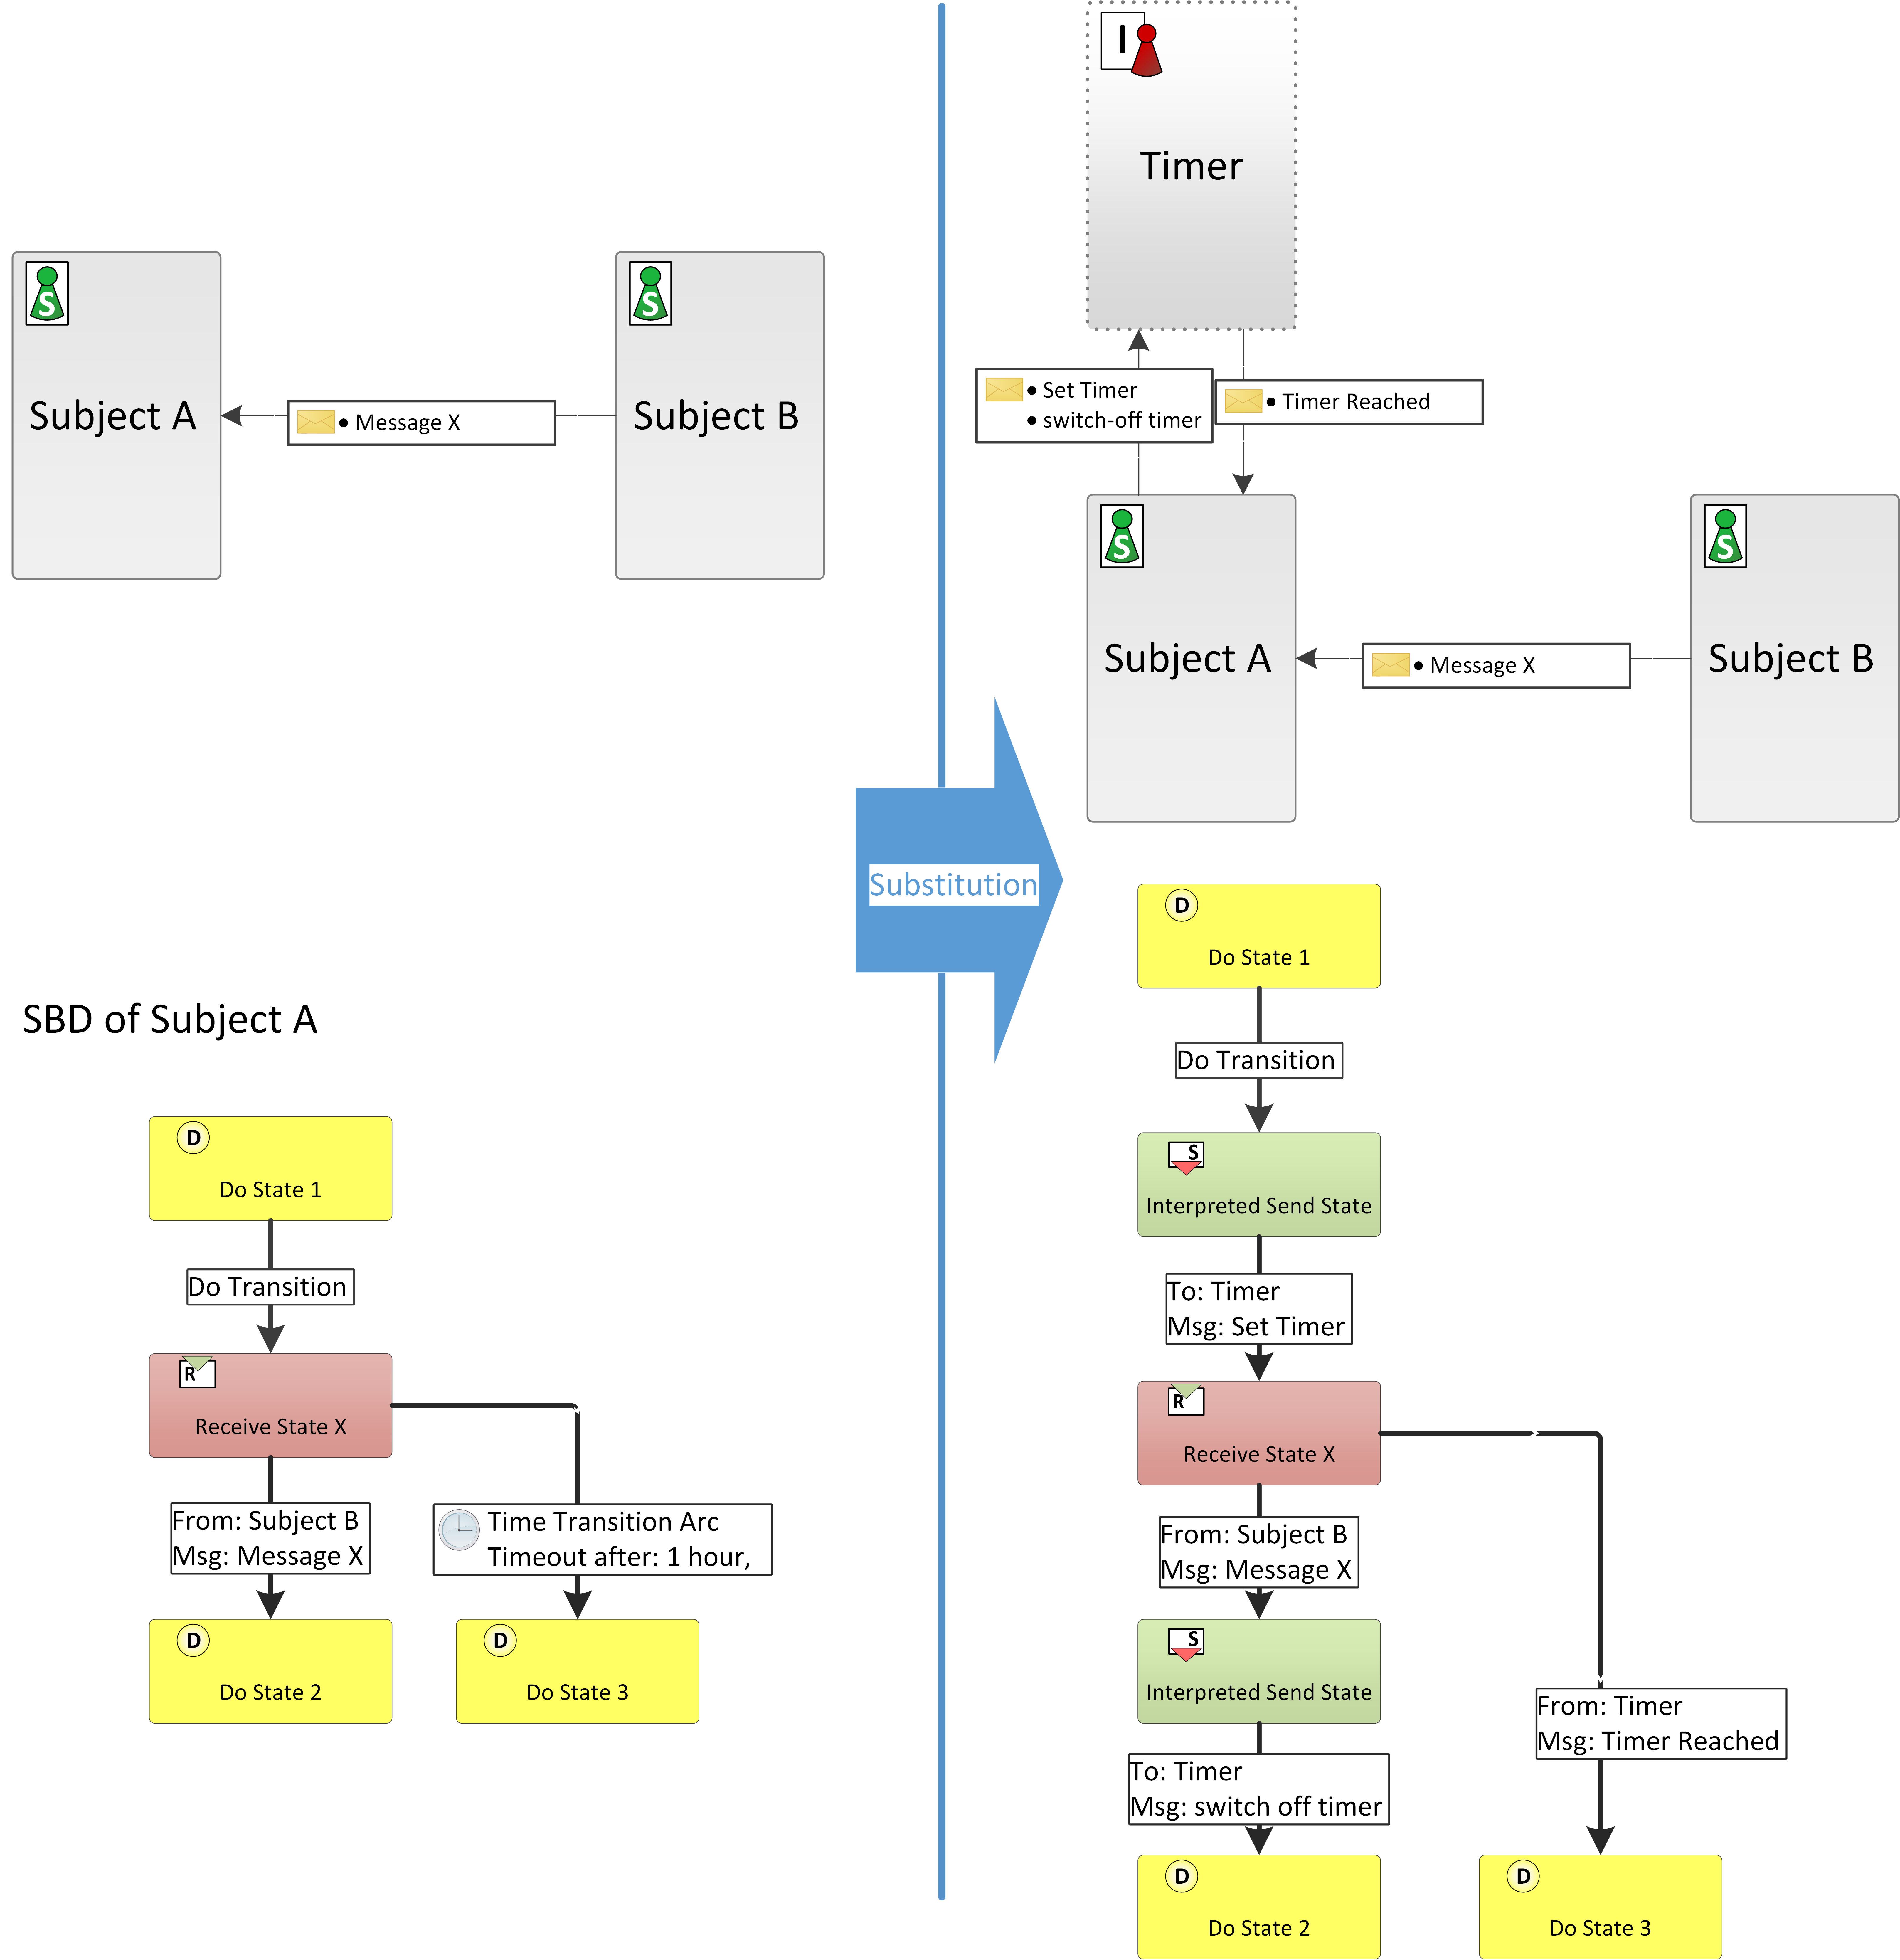
\includegraphics[width=1.0\linewidth]{Figures/Ontology/TimeOutReceiveStateInterpretationSIDSBD.png}
	\caption[Possible Substitution of \PASSModelElement{TimeOutTransiton}s from \PASSModelElement{Receive State}s for execution]{Possible Substitution of \PASSModelElement{TimeOutTransiton}s from \PASSModelElement{Receive State}s for execution}
	\label{fig:timeOutReceivesubstitution}
\end{figure*}

\emph{Timer from Send States}

Instead of setting a time with an assumed timer subject, a time-out transition originating from a send state is equal to a Sending Failed Transition with a modified time-out-time that is different from an execution environments default value. The Send Controller (see Section \ref{sec:sendingFailedTransitionsExecution}/ Figure \ref{fig:sendingfailedSubstituion}) simply needs to be informed about that specialized time-out time and send replies accordingly. 

\begin{figure*}[hp]
	\centering
	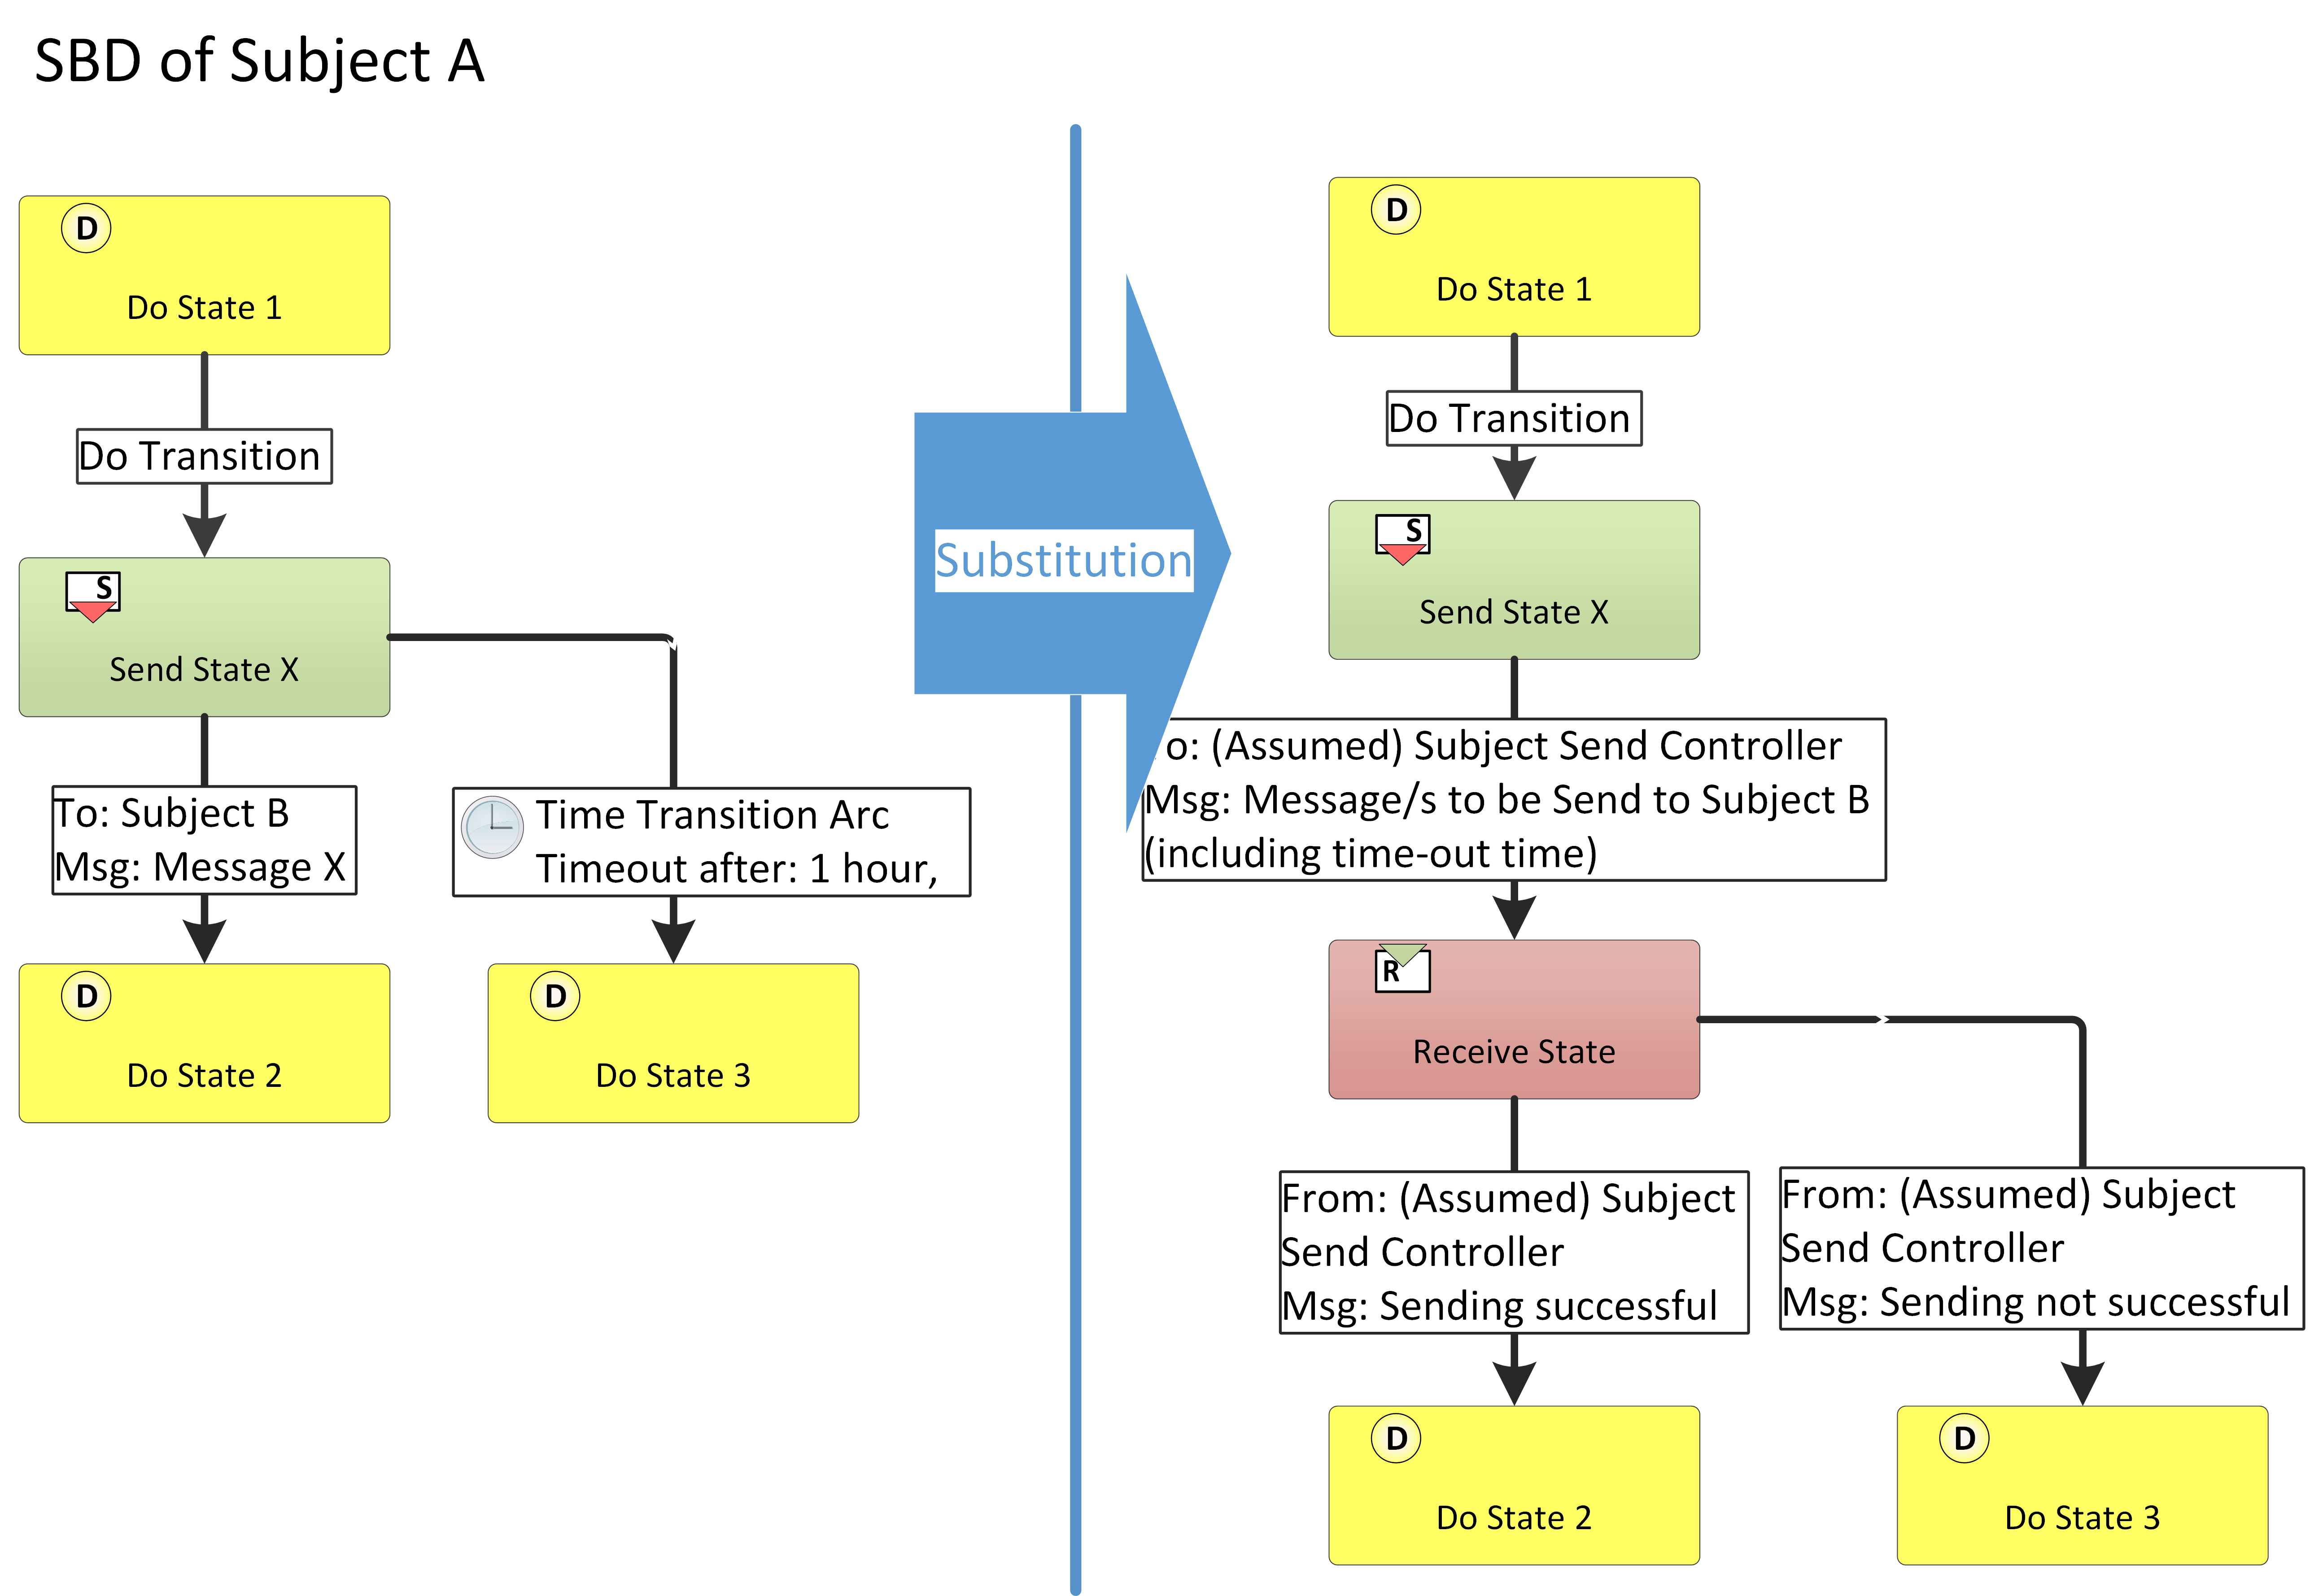
\includegraphics[width=1.0\linewidth]{Figures/Ontology/TimeOutSendStateInterpretationSBD.png}
	\caption[Possible Substitution of \PASSModelElement{TimeOutTransiton}s from \PASSModelElement{Send State}s for execution]{Possible Substitution of \PASSModelElement{TimeOutTransiton}s from \PASSModelElement{Send State}s for execution}
	\label{fig:timeOutSendSubstitution}
\end{figure*}

\emph{Timer from Do States}

Realizing time-outs for Do States is more complex. It could be done via a modification to that states internal Function Specification to include an additional internal time-out concept and substituting the outgoing Timer Transition with normal Do Transition that has the Transition Condition of  "time is up". 

A more complex substitution is shown in Figure \ref{fig:timeOutDoSubstitution}. Here, the concept of a Guard or Interrupt Behavior is employed, that guards only the single state that had the original time-out transition going out of it. The guard is triggered by a time-out message from a timer subject that needs to be set before entering the guarded state.

\begin{figure*}[hp]
	\centering
	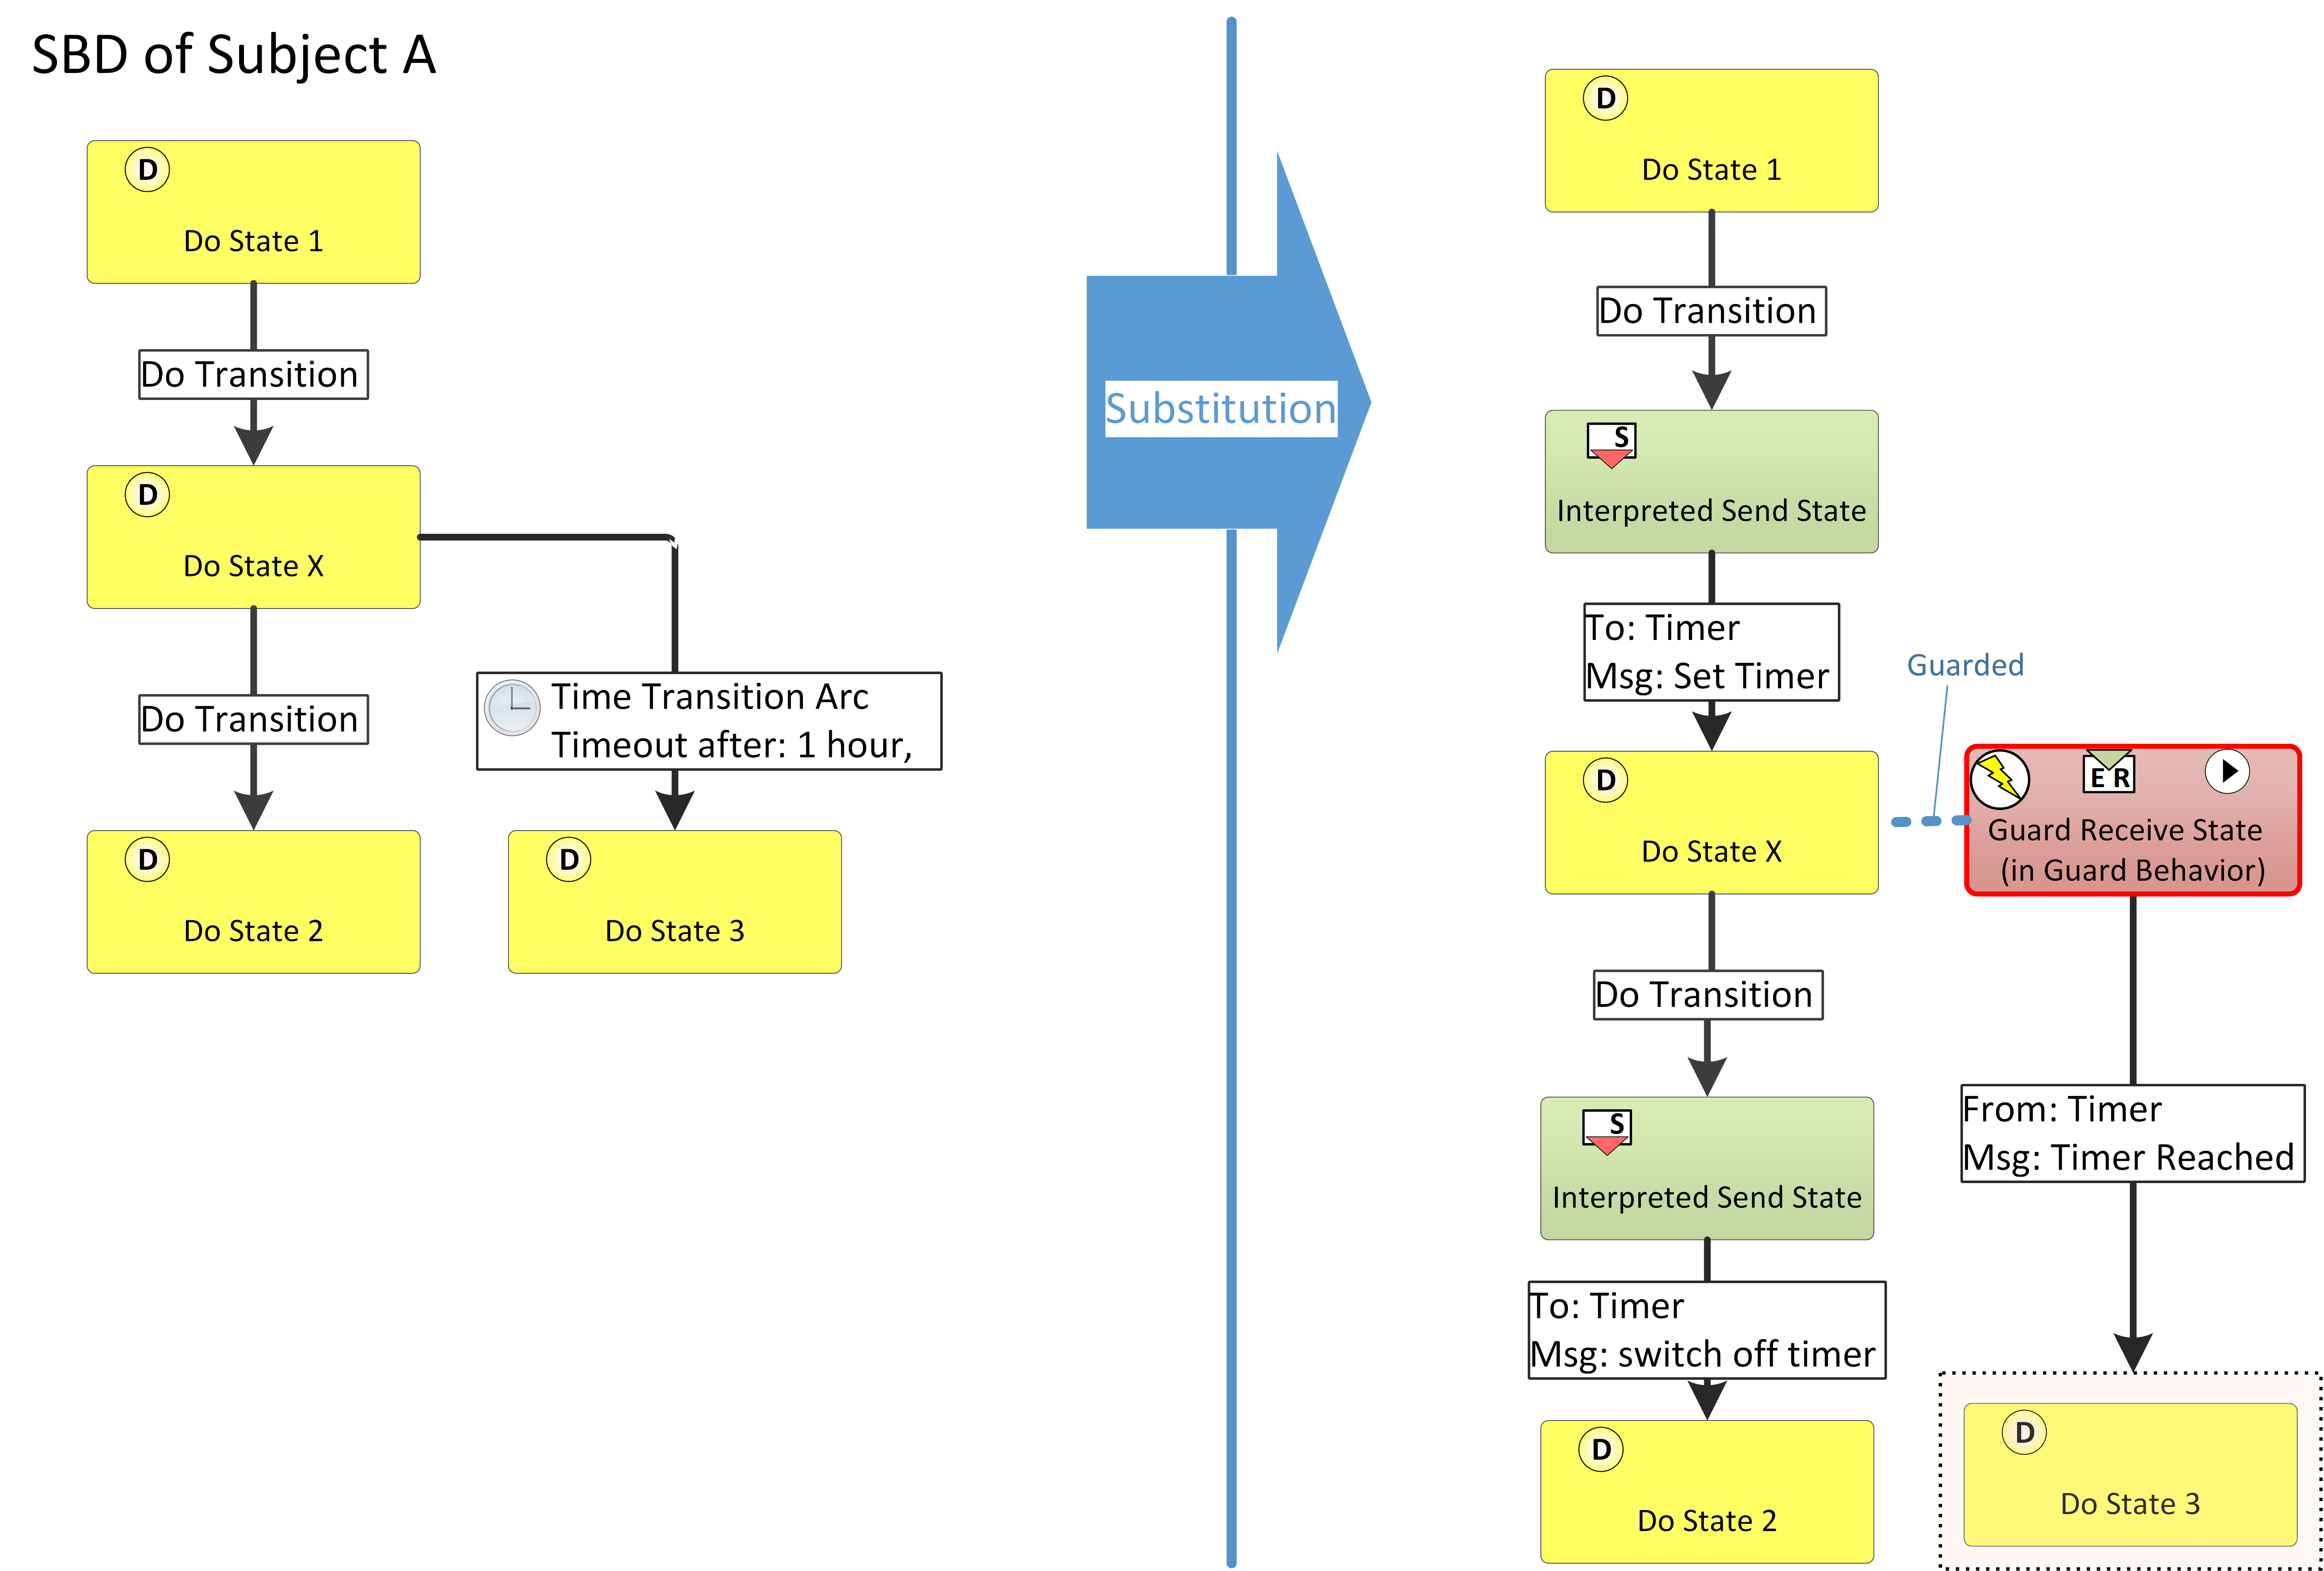
\includegraphics[width=1.0\linewidth]{Figures/Ontology/TimeOutDoStateInterpretationSBD.png}
	\caption[Possible Substitution of \PASSModelElement{TimeOutTransiton}s from \PASSModelElement{Do State}s for execution]{Possible Substitution of \PASSModelElement{TimeOutTransiton}s from \PASSModelElement{Do State}s for execution}
	\label{fig:timeOutDoSubstitution}
\end{figure*}

\subsubsection{Reminder Transitions}

Reminder Transitions are different from time-outs, as they are not triggered upon the passing of a specific amount of time after entering the state but rather, in terms of time since the transition has been traveled last or upon the passing of an calendar time interval.

Naturally, they are used only in States that will be (re-)visited multiple times and only \PASSModelElement{Receive States} and \PASSModelElement{Do States} are valid source states for these transitions.

Substitution is similar to that of Timer Transitions.  Again a Timer or Calendar Subject is assumed to exist, that is able to handle time based event calculation and send the according reminder messages upon reaching the time based conditions. Also, that timer needs to be set before entering the original source state for the first time. In contrast to a timer, the reminder message is send immediately so that transition could be traversed. In order to be able to send the next reminder correctly (be it 4 weeks or 4 seconds) the time must be informed if said transition has been followed as is shown in Figure \ref{fig:reminderReceiveSubstitution}. 


\begin{figure*}[hp]
	\centering
	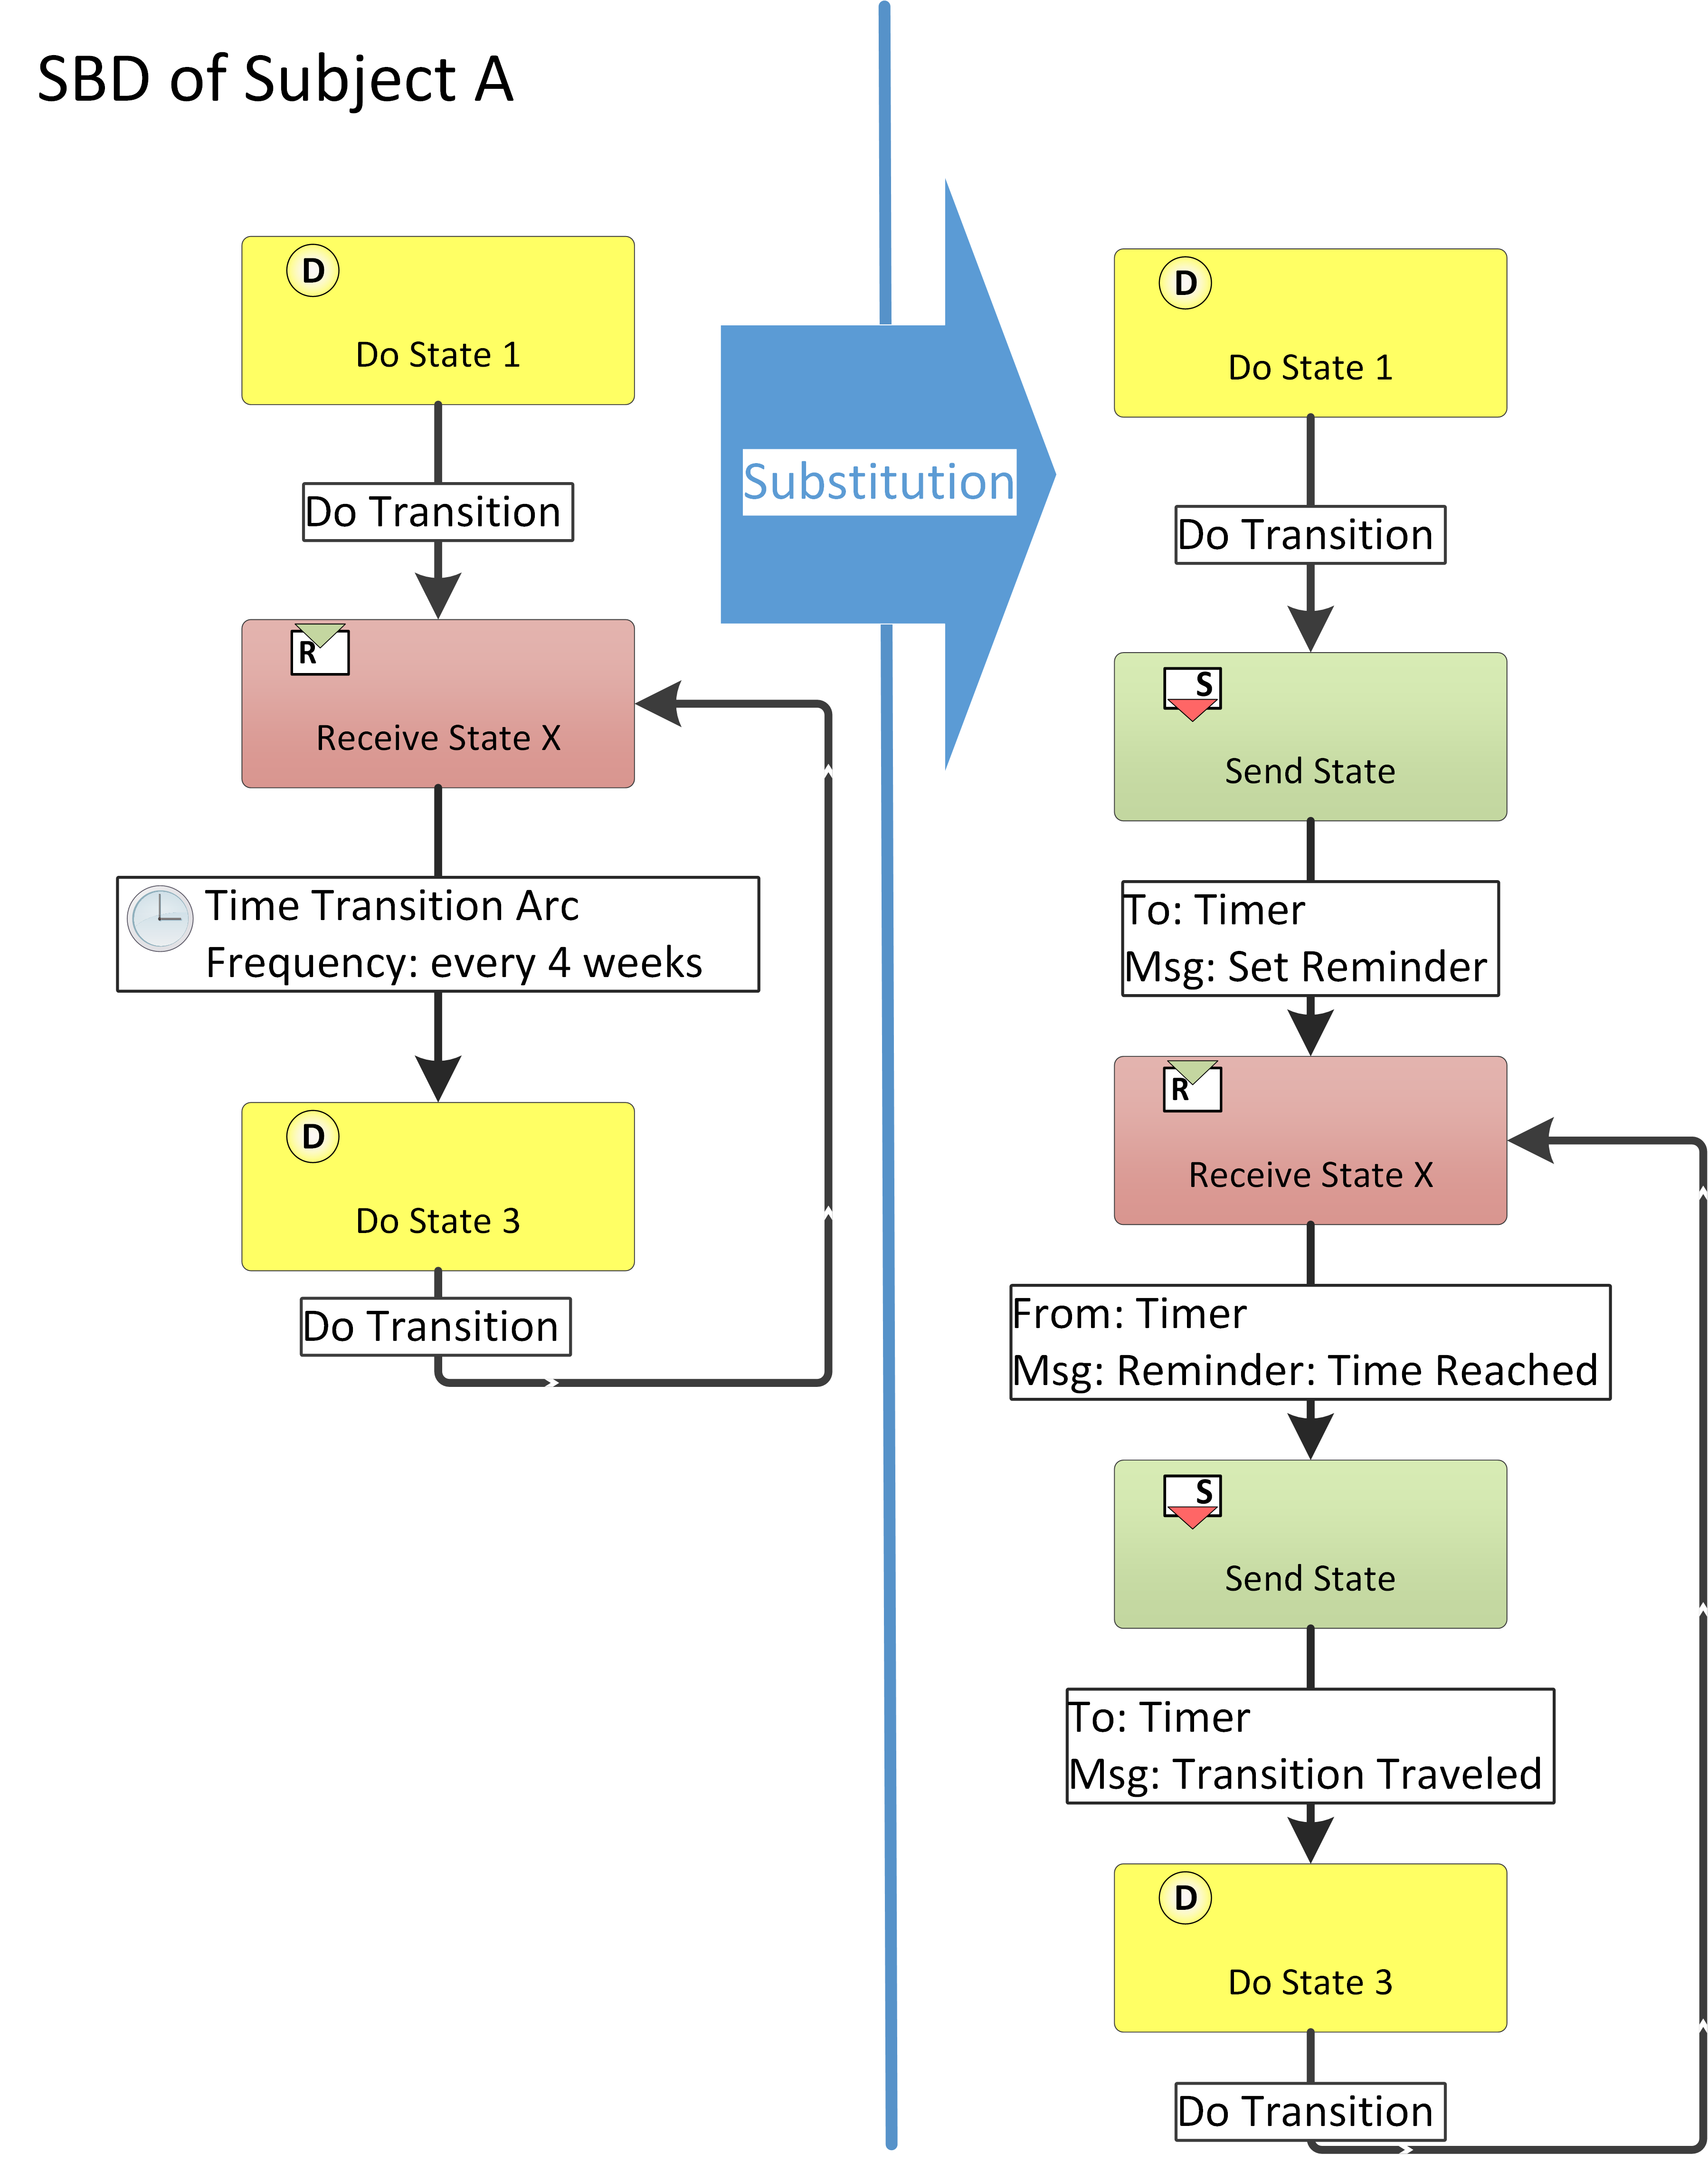
\includegraphics[width=1.0\linewidth]{Figures/Ontology/ReminderTransitionReceiveStateInterpretationSBD.png}
	\caption[Possible Substitution of \PASSModelElement{Reminder Transition}s from \PASSModelElement{Receive State}s for execution]{Possible Substitution of \PASSModelElement{Reminder Transition}s from \PASSModelElement{Receive State}s for execution}
	\label{fig:reminderReceiveSubstitution}
\end{figure*}

To keep the the number of reminder messages under Control an additional \PASSModelElement{Input Pool Restrictions} for that limits the number of reminder messages from that Timer Subject to one is useful, together with the \PASSDefaultIndividual{Input Pool Constraint Handling Strategy [of] Delete Oldest} for that message.




%The individual actions in the alternative paths of an alternative clause may be arbitrarily executed in parallel and overlapping (CS: interleving?), or in other words: A step can be executed in an alternative sequence, and then be followed by an action in any other sequence. This gives the performer of a subject the appropriate freedom of choice while executing his actions.

%In the example, the order can thus first be updated, and then the message 'order arrived' sent to sales. Now, either the message 'deliver order' can be sent to the warehouse or one of the internal functions, 'update sales status' or 'collect data for statistics', can be executed.

%The left alternative must be executed completely, and the middle alternative must also have been completed, if the first action ('inform sales' in the example) is executed. Only the left alternative can be processed because the middle one was never started. Alternatively, the sequence in the middle may have already reached its endpoint, while the left is not yet complete. In this case, the process waits until the left one has reached its endpoint. Only then will the state 'confirmation' be reached in the alternative clause. The right branch neither needs to be started, nor to be completed. It is therefore irrelevant for the completion of the alternative construct.


%ME: for now i have put all descriptions of SBD model elements into chapter 2b
%all aspects concerning execution are to be re put into this chapter


